\documentclass[11pt,oneside,openany]{book}
\usepackage[letterpaper,top=0.78in,bottom=0.82in,left=0.85in,right=0.85in,headheight=15pt]{geometry}
\usepackage[T1]{fontenc}
\usepackage{amsmath,amsthm,amssymb,mathtools}
\usepackage{mathpazo,microtype}
\usepackage{graphicx,float,booktabs,longtable,array,enumitem,xcolor,fancyhdr,titlesec,needspace,etoolbox,hyperref}
\definecolor{Ink}{HTML}{142D4E}
\definecolor{Accent}{HTML}{B08D57}
\hypersetup{colorlinks=true,linkcolor=Ink,citecolor=Ink,urlcolor=Ink,pdftitle={Machine-Native Reasoning: Reviewed Mathematical Core},pdfauthor={Komorebi P.},pdfsubject={Evidence, methods, and accountable revision}}
\setcounter{tocdepth}{0}
\hypersetup{bookmarksdepth=2}
\titleformat{\chapter}[display]{\normalfont\Large\bfseries\color{Ink}\hyphenpenalty=10000}{\chaptername\ \thechapter}{8pt}{\huge}
\titlespacing*{\chapter}{0pt}{0pt}{18pt}
\BeforeBeginEnvironment{theorem}{\begin{samepage}}
\AfterEndEnvironment{theorem}{\end{samepage}}
\BeforeBeginEnvironment{proposition}{\begin{samepage}}
\AfterEndEnvironment{proposition}{\end{samepage}}
\BeforeBeginEnvironment{corollary}{\begin{samepage}}
\AfterEndEnvironment{corollary}{\end{samepage}}
\BeforeBeginEnvironment{counterexample}{\begin{samepage}}
\AfterEndEnvironment{counterexample}{\end{samepage}}
\setlength{\parindent}{0pt}\setlength{\parskip}{5pt}\raggedbottom
\clubpenalty=10000\widowpenalty=10000\displaywidowpenalty=10000\emergencystretch=1em
\setlist{nosep,leftmargin=1.6em}
\renewcommand{\baselinestretch}{1.04}
\pagestyle{fancy}\fancyhf{}\fancyhead[L]{\small\scshape Machine-Native Reasoning}\fancyhead[R]{\small Reviewed Mathematical Core}\fancyfoot[C]{\thepage}
\fancypagestyle{plain}{\fancyhf{}\fancyfoot[C]{\thepage}\renewcommand{\headrulewidth}{0pt}}
\newtheorem{theorem}{Theorem}[chapter]
\newtheorem{proposition}[theorem]{Proposition}
\newtheorem{corollary}[theorem]{Corollary}
\theoremstyle{definition}\newtheorem{definition}[theorem]{Definition}
\newtheorem{counterexample}[theorem]{Counterexample}
\newcommand{\TV}{d_{\mathrm{TV}}}
\newcommand{\im}{\operatorname{im}}
\newcommand{\Span}{\operatorname{span}}
\newcommand{\Pow}{\mathcal P}
\newcommand{\source}[1]{\par{\small\textit{Source relationship.} #1}\par}
\newcommand{\boundary}[1]{\par{\small\textit{Boundary.} #1}\par}
\newcommand{\question}[1]{\par\medskip{\large\bfseries #1}\par\smallskip}
\begin{document}
\frontmatter
\hypersetup{pageanchor=false}
\begin{titlepage}
\thispagestyle{empty}
{\small\scshape REALIZATION CALCULUS\hfill MATHEMATICAL REASONING}\par
\vspace*{1.05in}
{\color{Ink}\fontsize{36}{41}\selectfont\bfseries Machine-Native\\[3mm]Reasoning\par}
\vspace{0.32in}
{\fontsize{20}{27}\selectfont Evidence, Methods,\\and Accountable Revision\par}
\vspace{0.38in}{\color{Accent}\rule{1.9in}{2pt}}\par
\vspace{0.38in}{\Large Komorebi P.\par}
\vfill
{\Large Reviewed Mathematical Core\par}
\vspace{0.25in}
{\large A continuous argument from accessible evidence to probability-valid operations, correction, controlled inquiry, and accountable revision.\par}
\vspace{0.32in}
Only the selected mathematical statements developed here belong to this core. The formal companion records their exact hypotheses and source correspondence. The wider research monograph has its own scope and review record.\par
\vspace{0.5in}
{\color{Ink}\rule{\linewidth}{0.7pt}}\par
{\small Selected results, complete written proofs, and formal correspondence\par}
{\small Original prose and figures: \href{https://creativecommons.org/licenses/by/4.0/}{Creative Commons Attribution 4.0 International}.\par}
\end{titlepage}
\hypersetup{pageanchor=true}
\chapter*{The shape of the argument}\addcontentsline{toc}{chapter}{The shape of the argument}
A machine can retain an answer without retaining a method. It can possess a method without having evidence to initialize it. It can execute that method correctly while using a record that no longer permits correction. It can improve one part of the computation while making the complete process more expensive. These are not unrelated qualifications. Each is a failure at a particular connection between evidence, representation, and action.

This book follows those connections in order. It begins with the information actually available to a reasoner. It asks what state that information can initialize, which operations the state supports, what must be remembered when further evidence arrives, and how one bounded investigation can acquire what is missing. Only then does it discuss improving the investigation and maintaining commitments across several participants.

The running example is deliberately small. A sensor reports a physical bit under an unknown convention, with a third nuisance bit that never affects the specified task. The example is enlarged only when a chapter explicitly changes its contract. It is not a model of a whole mind. Its purpose is to make hidden information, permitted actions, and each passage between results inspectable.

\begin{center}\begin{tabular}{>{\raggedright\arraybackslash}p{0.08\linewidth}>{\raggedright\arraybackslash}p{0.38\linewidth}>{\raggedright\arraybackslash}p{0.43\linewidth}}\toprule
Chapter & Question answered & What the next chapter still needs\\\midrule
1 & What does the record determine? & Operations that can be performed on the retained state.\\
2 & What survives a change of representation? & A record capable of later correction.\\
3 & What must memory retain? & Decisions and recipients that use that memory.\\
4 & What can the retained information justify? & An investigation that can actually acquire it.\\
5 & What fits one executable budget? & A justified way to improve the discovery procedure.\\
6 & What search work can be removed? & Evidence that remains applicable after a revision.\\
7 & Which guarantees and gains survive change? & Explicit treatment of other participants and obligations.\\
8 & What can be maintained together? & A clear boundary between the proved chain and its applications.\\\bottomrule
\end{tabular}\end{center}

The second admission block joins the signal-model, Bayesian-refinement, and artifact-planning sources at their common probability interface. Chapters 2, 3 and 5 are expanded in place: no whole source manuscript is appended.

There is one notation and one proof sequence. Repeated source arguments appear once. Original source names identify provenance, not new modules assumed to interoperate. The chapter endings explain exactly which output becomes the next chapter's input.

\chapter*{What the review label means}\addcontentsline{toc}{chapter}{What the review label means}
The earlier 1,919-page collection preserved source documents and navigation. Its own assembly report did not claim a proof review of every imported page. It remains a historical source reader. This book replaces breadth as the admission rule with result-level inspection.

A formal statement is admitted here only when its domains and quantifiers are explicit, its proof is given in full, its source relationship is identified, its use in a later chapter is checked, and its applicable finite construction or sharp boundary is exercised by a documented exact check. This is an internal mathematical review. It does not convert a finite check into a proof of an infinite statement.

The review is also narrower than accepting a source wholesale. A theorem selected from \emph{Machine Societies} does not import a general claim about spontaneously formed institutions. A linear reconstruction argument does not certify an emergent workspace. A commuting equation does not establish that a neural network learned its terms. Those stronger interpretations are outside the core.

The written statements and proofs in this reader retain their authenticated reviewed-core source. The formal companion records the corresponding Lean declarations, source-facing hypothesis checks, and reproducible verification gates. The formal correspondence chapter distinguishes those checks from the earlier finite computational receipts and from the wider research monograph. A formal counterpart applies to its stated mathematical contract; it does not establish that an implementation has learned or deployed that contract.

The companion review files name every retained result, its assumptions, its source anchor, its computational check, and its remaining limit. They also account for every source document in the former collection. Omission means either that its full evidence was not re-established for this edition or that it is unnecessary to the continuous argument. It is not a claim that the omitted work is false or valueless.

\tableofcontents
\mainmatter
\chapter{From evidence to a reusable state}\label{ch:evidence}
\question{The first question is not how much state to store. It is which distinctions are accessible.}
Let $\Omega$ be a finite nonempty set of possible worlds. A world may include a physical state, a fixed model index, and an origin tag. An observation record is a function $r:\Omega\to H$. A target is a function $t:\Omega\to Y$. All codomains used below are nonempty. We work on attained records $r(\Omega)$, so no arbitrary interpretation of an impossible record is needed.

\begin{proposition}[A record determines a target exactly on its fibres]\label{r:factor}
There exists $d:r(\Omega)\to Y$ with $d(r(\omega))=t(\omega)$ for every world if and only if
\[
r(\omega)=r(\omega')\ \Longrightarrow\ t(\omega)=t(\omega').
\]
\end{proposition}
\begin{proof}
Necessity follows because a function assigns one value to one input. For sufficiency, define $d(h)$ to be $t(\omega)$ for any world with $r(\omega)=h$. Such a world exists for attained $h$, and the hypothesis makes the choice immaterial. The resulting decoder satisfies the required equation.
\end{proof}
\source{Grounded Abstraction [GA], Proposition 3.2 and Theorem 3.4; Machine Understanding [MU], the representation and sender-access criteria. This is the shared elementary factorization argument, stated once.}

The proposition is an information statement, not a runtime bound. The table defining $d$ could be large. Nor does the mere existence of $d$ teach a learner how to find it. A proof that a suitable decoder exists and a justified account of its acquisition remain separate.

\section{The sensor used throughout the book}
Write a world as
\[
\omega=(b,s,n)\in\{0,1\}^3.
\]
The physical target bit is $b$. The sensor convention is $s$. The nuisance bit $n$ never affects the operations or outputs of the initial contract. The display is
\[
y=b\oplus s,
\]
where $\oplus$ is addition modulo two. A permitted control $f$ flips the physical bit and leaves $s,n$ unchanged. Consequently the next display is $1-y$.

An agent given only $y$ can predict every future display under repeated flips: after $k$ flips it is $y\oplus(k\bmod2)$. It cannot determine the current physical bit. Worlds $(0,0,0)$ and $(1,1,0)$ share display zero and have different targets. The obstruction is the fibre of the available record, not a shortage of computational effort.

Calibration is a separate, nondestructive observation $c(\omega)=s$. When calibration is permitted and trustworthy, the joint record $(y,s)$ determines $b=y\oplus s$. Adding a blank field called ``sensor convention'' does not provide this information. The observation operation, its interpretation, and its cost must be part of the contract.

\begin{center}\begin{tabular}{llll}\toprule
Available record & Number of values & Determines display? & Determines physical bit?\\\midrule
$y$ & 2 & Yes & No\\
$(y,s)$ & 4 & Yes & Yes\\
$(b,s,n)$ & 8 & Yes & Yes, with unused detail\\\bottomrule\end{tabular}\end{center}

\begin{figure}[ht]
\centering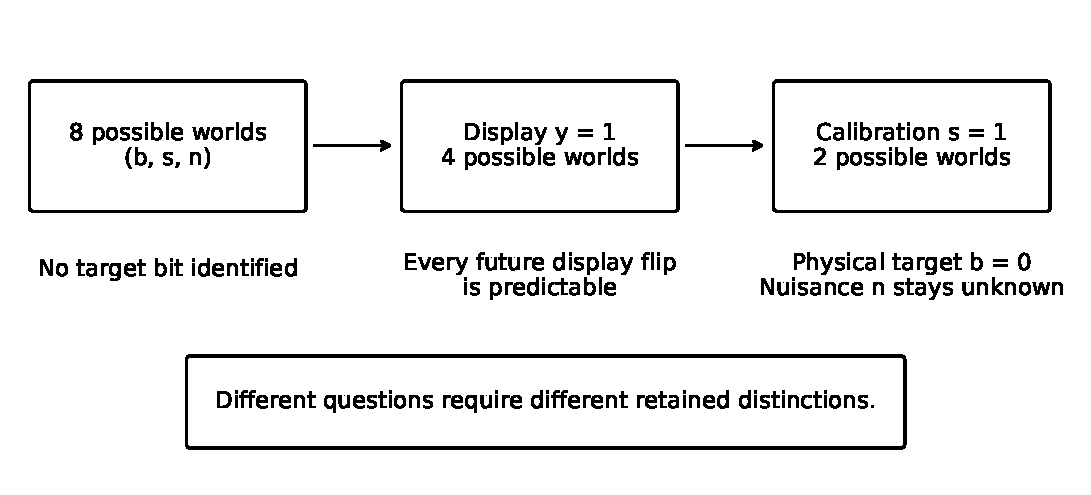
\includegraphics[width=\linewidth]{figures/sensor_chain.pdf}
\caption{One exact observation sequence. The last two worlds differ only in the nuisance bit. Knowing every hidden coordinate is unnecessary for the protected physical target.}
\end{figure}

\section{One answer versus every permitted continuation}
Let $X$ be a finite nonempty state space. Let $\mathcal A$ be a finite alphabet of total deterministic operations $F_a:X\to X$, and let $q:X\to Y$ be the protected output. A word $w=a_1\cdots a_k$ executes $a_1$ first. Thus $F_w=F_{a_k}\cdots F_{a_1}$, and the empty word denotes the identity.

Define behavioral equivalence by
\[
x\sim x'\quad\Longleftrightarrow\quad q(F_wx)=q(F_wx')\text{ for every finite word }w.
\]
The empty word protects the present output. The other words protect its permitted future uses.

\begin{theorem}[Evidence-initialized behavioral state]\label{r:behavior}
A finite predictor initialized only from $r(x)$, updated only by the operation names, and exact for all protected continuation outputs exists if and only if
\[
r(x)=r(x')\ \Longrightarrow\ x\sim x'.
\]
When it exists, $X/{\sim}$ supplies a predictor with the smallest possible number of initialized states. Its updates are $\bar F_a([x])=[F_ax]$ and its readout is $\bar q([x])=q(x)$.
\end{theorem}
\begin{proof}
If two initial records are equal, a deterministic predictor has the same initialized state. Applying the same subsequent operations produces the same predicted outputs. Exactness therefore requires behavioral equivalence.

For the converse, equivalent states have equivalent successors: an output after $F_a$ followed by $w$ is one of the outputs in the defining family. Hence $\bar F_a$ is well defined. The empty word makes $\bar q$ well defined. The fibre premise gives a well-defined initializer $d(r(x))=[x]$. Induction on word length proves exactness. Finally, behaviorally distinct states cannot initialize the same predictor state, since some continuation separates their outputs. Every exact predictor therefore needs at least one initialized value for each class, and the quotient attains that number.
\end{proof}
\source{[GA], Theorem 3.4, and [MU], Theorem 4.1. The two source versions are consolidated, not counted as independent discoveries.}

In the sensor, the display task has two behavioral states. Changing the protected output to $(y,b)$ yields four behavioral states. The old record still has only two values and cannot initialize the enlarged quotient. The new task has exposed a real information requirement.

\section{Why a statistical law is not an observed record}
A parameter can determine a distinct probability law while every finite sample remains possible under several parameters. For instance, Bernoulli parameters $1/3$ and $2/3$ assign positive probability to every finite binary string. No estimator based on one such string can be certainly correct for both parameters. The laws differ, but their finite supports overlap.

A correct uncertainty record can be the appropriate output in this setting. Calling the most probable world ``identified'' would silently replace an error-free claim with a probabilistic one. Chapter~\ref{ch:memory} gives the corresponding probability update explicitly.

\section*{What is now available}
We have a criterion for an initialized predictive state, but no automatic guarantee that an arbitrary coordinate manipulation preserves it. The next chapter studies operations on a representation. Its input is a declared state map and operation family, not an assumed learned encoder.

\chapter{Operations must survive their representations}\label{ch:operations}
\question{A representation is useful only to the extent that its intended operations remain meaningful.}
There are two different ways to change representation. An exact split representation retains the whole mathematical state in another space. A compression retains only part of it. The first can preserve arbitrary composition. The second needs additional conditions.

\section{Exact packets and the hidden-return defect}
Let $V,Z$ be vector spaces over a field. Let $A:V\to Z$ be analysis and $S:Z\to V$ synthesis, with $SA=I_V$. Then $AS$ is an idempotent on $Z$. The map $\mathcal E(T)=ATS$ represents a full-state operator $T:V\to V$ on resolved coordinates. Direct multiplication gives
\[
\mathcal E(T)\mathcal E(U)=ATSAUS=ATUS=\mathcal E(TU).
\]
The resolved identity is $AS$ on the compatible image $A(V)$, not necessarily $I_Z$ on arbitrary coordinates.

For a compression, reverse the splitting. Let $C:V\to Z$ and $R:Z\to V$ satisfy $CR=I_Z$, and put $P=RC$. The compressed operator is $\Phi(T)=CTR$.

\begin{proposition}[Exact accounting of the discarded excursion]\label{r:packet}
For any endomorphisms $T,U$ of $V$,
\[
\Phi(TU)-\Phi(T)\Phi(U)=CT(I-P)UR.
\]
Thus compression preserves this composition precisely when the discarded excursion on the right vanishes. Full split encoding $T\mapsto ATS$ preserves composition without that extra condition.
\end{proposition}
\begin{proof}
Expand the product $\Phi(T)\Phi(U)=CTRCUR=CTPUR$ and subtract it from $CTUR$. The identity for full split encoding follows from $SA=I_V$ as computed above. These computations make no approximation and require no orthogonality.
\end{proof}
\source{Sufficient Resolution [SR], Theorems 2.1 and 2.3. The present proof reviews only these algebraic identities, not the complete forty-seven-page source or its full formal implementation.}

\begin{counterexample}[A discarded coordinate returns]\label{ce:return}
Take $V=\mathbb R^2$, let $C(x_1,x_2)=x_1$, let $R(z)=(z,0)$, and let $T(x_1,x_2)=(x_2,x_1)$. The compressed one-step map is zero. Yet $T^2=I_V$, so $\Phi(T^2)=I_Z$, while $\Phi(T)^2=0$. The discarded second coordinate was not irrelevant to the two-step question.
\end{counterexample}

This is the mathematical reason that a short successful readout is not enough. A representation may preserve what is visible now and lose a route by which hidden information becomes visible later. Packets identify the retained and residual components, but the decomposition alone does not prove the residual harmless.

\section{A method can be transported without reconstructing everything}
Suppose source states $z\in Z$ have operations $F_a$, target states $u\in U$ have operations $G_{\tau(a)}$, and $T:Z\to U$ is a translation. The operation-name map $\tau$ is fixed. Let $q$ and $\bar q$ be matched readouts.

\begin{theorem}[Forward transport of a reusable method]\label{r:transport}
If the source domain is invariant, and
\[
TF_a=G_{\tau(a)}T,\qquad q=\bar qT,
\]
then for every finite word $w$,
\[
TF_w=G_{\tau(w)}T,\qquad qF_w=\bar qG_{\tau(w)}T.
\]
\end{theorem}
\begin{proof}
The empty word gives $TI_Z=I_UT$. Assume the first equality for a prefix. Invariance allows the next local equality to be applied on its successor, yielding
$TF_aF_w=G_{\tau(a)}TF_w=G_{\tau(a)}G_{\tau(w)}T$.
Induction proves the first claim. Composition with the matched readout proves the second.
\end{proof}
\source{[MU], Theorem 6.1; the same local-to-continuation argument appears in OSL and Neuralese. No claim about a learned latent translator is imported.}
\boundary{The theorem is forward. It does not imply an inverse, matching of new target operations, cheap computation of $T$, or that the source solver causally uses the represented state.}

The sensor representation $(y,s)$ translates to $(b,s)$ through $T(y,s)=(y\oplus s,s)$. Flipping the physical bit complements the first coordinate in either representation. The square commutes, and so does every repeated flip. The nuisance bit is never reconstructed because it has no role in this contract.

\section{One quotient for several possible dynamics}
A stronger situation arises when the operator itself is uncertain. Let $V$ be finite dimensional, let $T_a^\theta$ be finitely many candidate linear operators, and let $A_a$ be one complete candidate system chosen as reference. A model index $\theta$ is fixed during the initial comparison. Let $Q:V\to Y$ be the same linear readout for every candidate.

Define $D_a^\theta=T_a^\theta-A_a$ and the propagated discrepancy space
\[
E=\Span\{A_wD_a^\theta v: v\in V,\ a,\theta,\ w\text{ finite}\}.
\]
It can be constructed by starting with the sum of the discrepancy ranges and repeatedly adding their images under the reference actions. In finite dimension this increasing sequence stops. Immediate invisibility $QD_a^\theta=0$ alone does not guarantee $QE=0$.

\begin{theorem}[A common observable quotient]\label{r:common}
The following conditions are equivalent:
\begin{enumerate}
\item $QT_w^\theta=QA_w$ on all of $V$, for every fixed candidate $\theta$ and every word $w$.
\item $E\subseteq\ker Q$.
\item There is a surjective linear $r:V\to Z$, common updates $G_a$, and a readout $\bar Q$ with $rT_a^\theta=G_ar$ and $Q=\bar Qr$ for every $a,\theta$.
\end{enumerate}
Under these conditions, $V/E$ is a common quotient and also predicts the output when the candidate index changes between operations.
\end{theorem}
\begin{proof}
Assume the first condition. For every $a,\theta,w$, equality as operators on all of $V$ gives
\[
QA_wD_a^\theta=QT_w^\theta T_a^\theta-QA_wA_a=0.
\]
The last equality applies the premise to the word executing $a$ and then $w$. Spanning proves $E\subseteq\ker Q$.

Conversely, $E$ is invariant under every $A_a$ by construction, and contains the entire range of each difference $D_a^\theta$. Hence $T_a^\theta E\subseteq E$, and every candidate induces the same map $G_a([v])=[A_av]$ on $V/E$. Since $QE=0$, the readout descends. This proves the third condition. Composing its equalities yields the first condition. The same induction permits a different $\theta$ at each step because the quotient map and update remain shared.
\end{proof}
\source{[GA], Theorem 13.1, ``Exact common quotient for structured model uncertainty.'' The all-initial-vectors hypothesis is retained.}

For example, let $Q(x_1,x_2,x_3)=x_1$ and let every candidate act as
\[
T^\theta(x_1,x_2,x_3)=(x_1+x_2,x_2,\theta x_3).
\]
Then $E$ is contained in the third coordinate and remains invisible. The two-coordinate method $(x_1,x_2)\mapsto(x_1+x_2,x_2)$ is exact, although the hidden dynamics are not identified.

The conclusion would be different if a later action moved the third coordinate into the first. That change enlarges $E$ beyond $\ker Q$. It invalidates the use of this quotient, not the theorem that justified the former one.


\section{An algebraic packet is not automatically a probability}
The previous sections concern linear representations. Bayesian correction will require more: a nonnegative state with a well-defined total mass. Those requirements belong to a declared domain, not to the spelling of its coordinates.

Let $\mathcal K$ be a convex cone in a real vector space, and let $\lambda$ be linear and strictly positive on every nonzero member of $\mathcal K$. Its normalized states satisfy $v\in\mathcal K$ and $\lambda v=1$. A coordinate change can send $\mathcal K$ to a cone containing negative coordinates without changing those states' probability meaning. Conversely, an arbitrary signed component of a valid state need not itself be valid.

\begin{proposition}[When complete packets are genuine probability components]\label{r:positive-packets}
Let $P_1,\ldots,P_m$ be linear maps with $\sum_iP_i=I$. If every $P_i$ preserves $\mathcal K$, each normalized $v\in\mathcal K$ has the mixture decomposition
\[
 v=\sum_{i:w_i>0}w_i v_i,\qquad
 w_i=\lambda P_iv\ge0,\quad \sum_iw_i=1,\quad v_i=P_iv/w_i.
\]
Every zero-weight component is zero. If $\mathcal K=\mathbb R^d_{\ge0}$ and the $P_i$ are also idempotent, they must be disjoint diagonal coordinate selections. Orthogonal completeness alone does not imply a probability mixture.
\end{proposition}
\begin{proof}
Cone preservation places $P_iv$ in $\mathcal K$, so its mass is nonnegative. Strict positivity says that a member of this cone with zero mass is zero. Applying $\lambda$ to the complete decomposition gives $\sum_iw_i=\lambda v=1$. Dividing every nonzero component by its mass proves the mixture identity.

On the nonnegative coordinate cone, preservation is equivalent to nonnegative matrix entries, as is seen by applying a matrix to every standard basis vector. Because the matrices sum to $I$, their nonnegative off-diagonal entries must all vanish. An idempotent diagonal entry satisfies $x^2=x$, hence is zero or one. The diagonal sums are one, so each coordinate is selected by exactly one map. Finally, completeness and orthogonality without positivity do not give the first premise, as the following example shows.
\end{proof}
\source{Large Signal Model Foundations [LSM], Proposition 30, physical page 40. Only this finite packet argument and the joint-closure result below are admitted from that source at this stage.}

\begin{counterexample}[An exact detail component has negative probability mass]\label{ce:signed-packet}
For $p=(3/4,1/4)^\top$, the orthogonal average and detail projectors are
\[
 P_{\rm av}=\tfrac12\begin{pmatrix}1&1\\1&1\end{pmatrix},\qquad
 P_{\rm det}=\tfrac12\begin{pmatrix}1&-1\\-1&1\end{pmatrix}.
\]
They sum to the identity and produce $(1/2,1/2)^\top$ and $(1/4,-1/4)^\top$. The components reconstruct $p$ exactly, but the detail has zero total mass without being zero. Normalizing it as a belief is undefined. Clipping its negative entry and normalizing the resulting sum would instead produce $(3/5,2/5)^\top$, a different belief.
\end{counterexample}

\begin{figure}[ht]
\centering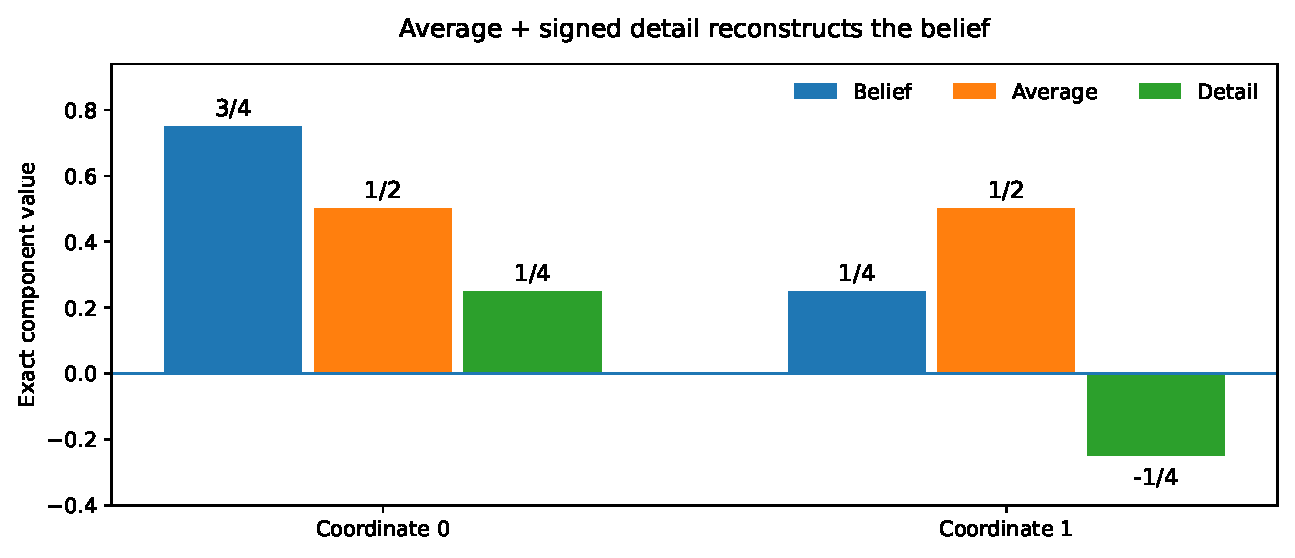
\includegraphics[width=.92\linewidth]{figures/signed_packets.pdf}
\caption{Exact reconstruction and probability interpretation are different requirements. The signed detail is useful algebraically but is not a separate probability distribution. Values are from Counterexample~\ref{ce:signed-packet}.}
\end{figure}

This distinction supplies the interface to the next chapter. A signal packet may describe a discrepancy, a coordinate, or a component of an operator. A belief represents nonnegative mass over alternatives. Moving between them requires a domain-preserving map. No learned signal architecture is inferred from this algebraic admission.

\section*{What is now available}
We have a declared method that preserves the selected outputs. But a predictive quotient need not retain the relationships needed for new evidence. The next chapter changes the retained object from a current physical coordinate to a set or distribution of candidate worlds.

\chapter{Memory that remains open to correction}\label{ch:memory}
\question{A useful memory preserves the distinctions by which its own conclusions can be revised.}
Let $t:\Omega\to Y$ be the current target. A candidate set $V\subseteq\Omega$ records worlds still possible. The empty set is allowed and means that the represented candidates contradict the admitted evidence. It is not a successful identification.

Let $\mathcal E\subseteq\Pow(\Omega)$ contain $\Omega$ and be closed under intersection. In this chapter the world does not change when an evidence event is received. The update is $V\mapsto V\cap E$. Physical actions and their effects will return in Chapter~\ref{ch:inquiry}.

\section{A state sufficient for every later filter}
Define the correction signature
\[
\Sigma(V)=\bigl(t(V\cap E)\bigr)_{E\in\mathcal E}.
\]
It records what each admitted future filter would leave of the possible target values.

\begin{theorem}[Minimal exact memory for a correction contract]\label{r:memory}
Equality of $\Sigma$ is a congruence for every update $V\mapsto V\cap E_0$. The signature supports the current target set and its exact update after every finite evidence sequence. Any deterministic retained state supporting the same readouts and updates on all candidate subsets must distinguish every two distinct signatures. Thus the image of $\Sigma$ has the least possible cardinality for this contract.
\end{theorem}
\begin{proof}
If $\Sigma(V)=\Sigma(W)$, then for each $E$,
\[
t((V\cap E_0)\cap E)=t(V\cap(E_0\cap E))=t(W\cap(E_0\cap E)).
\]
Intersection closure supplies the coordinate $E_0\cap E$, so the updated signatures agree. The $\Omega$ coordinate is the present target set. Induction gives every finite sequence.

If signatures differ, one admitted event produces distinct target sets. A memory that merged those candidates would update identically and return the same answer on that event, contradicting exactness. Hence each signature needs its own state. The signature construction attains the lower bound.
\end{proof}
\source{[GA], Theorem 5.2. This is a behavioral quotient of the correction process, not a claim that all candidate sets must be stored literally.}

\section{An exact count for partition evidence}
Suppose $C_1,\ldots,C_m$ partition $\Omega$ into nonempty cells and the admitted events are \emph{exactly} their unions. Let
\[
D_t=\{(i,y): C_i\cap t^{-1}(y)\ne\varnothing\},\qquad r=|D_t|.
\]
The occupancy memory retains whether a candidate exists in each attainable cell--target pair.

\begin{corollary}[The size of partition correction memory]\label{r:occupancy}
On all subsets of $\Omega$, correction signatures are exactly distinguished by these occupancy records. There are $2^r$ signatures, and $r$ fixed binary bits are necessary and sufficient to encode them.
\end{corollary}
\begin{proof}
An individual-cell filter reveals the target values occupied in that cell, so the signature determines occupancy. Conversely, occupancy determines the target values left by any union of cells. Every subset of $D_t$ occurs: select one world from each included nonempty cell--target intersection and none from excluded intersections. Those intersections are disjoint. Thus there are precisely $2^r$ possible records. The preceding theorem and binary counting give necessity, while the occupancy vector supplies sufficiency.
\end{proof}
\source{[GA], Corollary 5.3. The word ``exactly'' in the evidence premise is essential.}

For the sensor, the four cells are fixed pairs $(b,s)$ with either nuisance value. Calibration and display evidence generate their unions. The target is $b$, so there are four attainable cell--target pairs. Candidate membership uses eight bits for eight worlds. Correction memory uses four bits for sixteen possible occupancies. The current target set alone has four possibilities and needs only two bits, but is not sufficient for later calibration.

For example,
\[
V=\{(0,0,0),(1,1,0)\},\qquad W=\{(0,1,0),(1,0,0)\}
\]
have the same possible target set $\{0,1\}$. After the event $s=0$, one leaves target zero and the other target one. Their different associations are operationally relevant.

\begin{counterexample}[A new evidence event changes the required memory]\label{ce:split}
Take one cell $\Omega=\{u,v\}$ and a constant target. The singleton candidate sets have the same old occupancy. If the event $\{u\}$ is added, filtering one singleton gives a target value while filtering the other gives contradiction. A record sufficient for the old event algebra is insufficient for the larger one.
\end{counterexample}

\section{Noisy correction is not elimination}
A likelihood can be small without being zero. Deleting a candidate because an observation was surprising can invalidate a correct noise model. We therefore specify a separate probability contract.

Let $M\in\mathcal M$ be a fixed model with prior $p(m)$. Let an experiment have likelihood $L_m(o)$ on a finite nonempty observation alphabet $\mathcal O$. A reporting channel $B(o,z)$, independent of the model conditional on $o$, creates a retained report $Z$. The joint law is
\[
\Pr(m,o,z)=p(m)L_m(o)B(o,z),\qquad Q_m(z)=\sum_oL_m(o)B(o,z).
\]
Posterior distributions are defined only on positive-probability events.

\begin{theorem}[When a report preserves every Bayesian correction]\label{r:bayes}
The following are equivalent:
\begin{enumerate}
\item For every prior, the posterior after $o$ equals that after $z$ on every positive-probability pair $(o,z)$.
\item The equality holds for one prior positive on every model.
\item There is a stochastic kernel $\rho(o\mid z)$ such that
\[
L_m(o)B(o,z)=Q_m(z)\rho(o\mid z)\quad\text{for all }m,o,z.
\]
\end{enumerate}
The reconstruction in the last condition refers to the actual joint experiment, not an unrelated simulation with matching marginals.
\end{theorem}
\begin{proof}
The first condition implies the second. Under a positive prior, define $\rho(o\mid z)=\Pr(o\mid z)$ whenever $z$ has positive probability. For a positive pair, posterior equality yields
\[
p(m)L_m(o)B(o,z)=\Pr(o,z)p(m\mid o)
=\rho(o\mid z)\Pr(z)p(m\mid z).
\]
Substituting Bayes' formula and cancelling positive $p(m)$ gives the factorization. A zero-probability pair under a positive prior has $L_m(o)B(o,z)=0$ for all $m$; its conditional weight is zero. If $z$ is impossible for every model, assign any probability row to $\rho(\cdot\mid z)$ because both sides vanish.

Conversely, the factorization makes the likelihood of $(o,z)$ a model-independent multiple of the likelihood of $z$. Normalization under any prior therefore gives $p(m\mid o,z)=p(m\mid z)$. Since the common channel only reads $o$, the same positive-pair posterior equals $p(m\mid o)$. This proves the first condition.
\end{proof}
\source{[MU], Theorem 12.1. The full-support and zero-probability cases are included in the proof.}

The theorem permits removal of an independent nuisance flag. It does not permit removal of every association. Consider two priors on $(b,s)$, with rows indexed by $b$ and columns by $s$:
\[
P=\begin{pmatrix}1/2&0\\0&1/2\end{pmatrix},\qquad
P'=\begin{pmatrix}0&1/2\\1/2&0\end{pmatrix}.
\]
Both individual marginals are uniform. A noisy calibration reports $s$ correctly with probability $3/4$, independently conditional on the fixed world. The probability of report one is $1/2$ under both priors. After that report, however, the target posteriors are $3/4$ and $1/4$. Separate target and sensor marginals cannot support this correction. Their association matters even though neither marginal changed.

These examples do not identify a universally optimal memory. They identify the least information required by a specified correction contract. A new likelihood, a newly admitted model, or a different target can change that requirement.


\section{A record must close under prediction as well as correction}
The static Bayesian theorem preserves one update of a fixed candidate model. A continuing reasoner also predicts what happens between observations. The same compressed record must support both operations. Otherwise a valid posterior can become an inadequate input to the very next prediction.

First consider a known finite state set $X$ with row-stochastic transition matrices $K_a(x,x')$. We retain column-vector probability distributions. A partition $\pi$ has aggregation $C_\pi(z,x)=1_{\{\pi(x)=z\}}$, so prediction is $p\mapsto K_a^\top p$. For each permitted observation symbol $o$, let $\ell_o(x)>0$ be its specified likelihood. When these are a complete report alphabet, assume also $\sum_o\ell_o(x)=1$.

A mandatory partition $\pi_0$ with at least two blocks protects the target distinctions. We seek a refinement that supports every prediction and each separate Bayesian update for every prior. The observation is an operation available in its own right. This is stronger than inspecting only a chosen combined transition-and-report schedule.

\begin{theorem}[Least refinement closed under prediction and correction]\label{r:joint-refinement}
First split $\pi_0$ by the complete vectors $(\ell_o(x))_o$, obtaining $\pi_{\rm init}$. Then repeatedly split current blocks by
\[
 \left(\sum_{x'\in B}K_a(x,x')\right)_{a,B},
\]
where $B$ runs over the current blocks. The process stops after at most $|X|-|\pi_{\rm init}|$ strict refinement rounds. Its final partition is the unique coarsest refinement of $\pi_0$ for which all specified predictions admit stochastic coarse transitions and all separate Bayesian updates admit fixed strictly positive coarse likelihoods for every prior.
\end{theorem}
\begin{proof}
At a stable partition the probability of reaching each coarse block depends only on the current block. These sums define a stochastic coarse transition and yield $C_\pi K_a^\top=\bar K_a^\top C_\pi$, first on point masses and then by linearity. Likelihoods are constant within final blocks. Grouping the numerator and normalizer by those blocks therefore commutes with every Bayesian update.

For minimality, take any admissible refinement $\eta$ of $\pi_0$. It has at least two blocks. Fix a strictly positive fine likelihood $\ell$ and a strictly positive coarse likelihood $\bar\ell$ inducing its assumed update. For states $x,y$ in one block and $z$ in a different block, compare priors assigning half their mass to $x,z$ and to $y,z$. Their coarse priors agree. Equality of the posterior odds gives
\[
 \ell(x)/\ell(z)=\bar\ell(\eta(x))/\bar\ell(\eta(z))=\ell(y)/\ell(z).
\]
Thus $\ell(x)=\ell(y)$, and $\eta$ refines the first likelihood split. Coarse likelihoods may differ by a positive scale for each observation without changing this conclusion.

If $\eta$ refines a current partition, each current block is a union of $\eta$ blocks. Exact prediction under $\eta$ makes the probability of reaching each such union constant inside every $\eta$ block. Hence $\eta$ refines the next split too. Induction proves that every admissible refinement refines the terminal one. Each strict round increases the block count, proving the bound. Coarseness determines the partition uniquely, up to naming its blocks.
\end{proof}
\source{[LSM], Proposition 9 and Proposition 12, physical pages 11--14; Bayesian necessity also appears in PRIQ [PRIQ], Theorem 5.6. The proof includes the two-block and strict-positivity premises rather than importing them by a cross-reference.}

For the sensor, the mandatory display partition has two blocks. A noisy calibration that reports $s$ correctly with probability $3/4$ splits it into the four $(b,s)$ blocks. The nuisance bit remains merged. The physical flip maps these four blocks among themselves, so the transition stage introduces no further split. The representation is now closed for both prediction and correction, not merely for today's display.

Refinement can also propagate backward through dynamics. In a separate four-state example, the mandatory partition is $\{0,1,2\}\mid\{3\}$ and the deterministic successors are $(0,2,3,3)$. A constant likelihood adds no information. Transition signatures first isolate state 2, then separate 0 from 1. The final partition is discrete. The reason for the second split is a future observable difference, not a newly sampled measurement.

The construction uses complete tables. It does not acquire those tables, certify their physical accuracy, or guarantee a finite encoding of every posterior coordinate. Its least-state statement concerns the specified separate operations and all priors. Different admissible schedules or reachable-prior restrictions can justify another quotient.

\section{Retain the joint law of the report and the next state}
A general experiment can change the state and report correlated information about the change. Describing its transition and report marginals separately is then insufficient. Let
\[
 K_{a,o}(x',x)=\Pr(X_{t+1}=x',O_{t+1}=o\mid X_t=x,A_t=a)
\]
be a nonnegative finite instrument with $\sum_{o,x'}K_{a,o}(x',x)=1$ for every $a,x$. This notation is column-oriented: $K_{a,o}p$ is an unnormalized post-experiment distribution. It specifies an experiment's physical change and its observation in one object.

For a surjection $\pi:X\to Z$, let $C$ sum probabilities over its fibres. Write
\[
 z_{a,o}(p)=\mathbf1^\top K_{a,o}p,\qquad
 \Psi_{a,o}(p)=K_{a,o}p/z_{a,o}(p)
\]
when the denominator is positive. Zero mass means an impossible report under that prior, not an arbitrarily assigned posterior.

\begin{theorem}[One quotient for reports, posteriors, and feedback]\label{r:instrument}
A nonnegative normalized coarse instrument $\bar K_{a,o}$ satisfies
\[
 CK_{a,o}=\bar K_{a,o}C\quad\text{for every }a,o
\]
if and only if, for all $a,o,z'$,
\[
 \sum_{x':\pi(x')=z'}K_{a,o}(x',x)
\]
is constant as $x$ varies within any one input fibre. Such a coarse instrument is unique. Equivalently, it preserves for every prior both the report probabilities and the aggregated positive-probability posteriors:
\[
 z_{a,o}(p)=\bar z_{a,o}(Cp),\qquad C\Psi_{a,o}(p)=\bar\Psi_{a,o}(Cp).
\]
Starting from $Cp_0$, these identities preserve every finite joint action/report law and every corresponding coarse posterior under one common policy that uses only the previously observed action/report history. This includes randomized policies with the same history-conditional action probabilities.
\end{theorem}
\begin{proof}
Applying the matrix identity to a point mass proves necessity of the fibre condition. Conversely, use the common sums to define each column of $\bar K_{a,o}$. They are nonnegative. Summing across $z',o$ partitions the fine successor set and gives column mass one. The definition proves the matrix equality on point masses, hence on every vector. Surjectivity gives uniqueness.

Because $\mathbf1_Z^\top C=\mathbf1_X^\top$, the matrix equality gives equal report masses. Dividing it by a common positive mass gives equal aggregated posteriors. Conversely, equality of masses and positive-mass posteriors gives the unnormalized matrix equality on every prior. If the common mass is zero, both unnormalized vectors are zero by nonnegativity. Point masses finish that direction.

For a history $h$, keep unnormalized states $u_h,\bar u_h$. Initially $\bar u_\varnothing=Cu_\varnothing$. After choosing action $a$ with common probability $\gamma(a\mid h)$ and receiving $o$, the next states are $\gamma(a\mid h)K_{a,o}u_h$ and $\gamma(a\mid h)\bar K_{a,o}\bar u_h$. The intertwining identity preserves their aggregation. Induction gives equal mass for every history, including zero-mass histories. Normalization on positive histories gives the posterior statement. Stopping decisions based on the same history can be included as matching terminal choices.
\end{proof}
\source{Selected synthesis of the positive-transfer and filtering arguments in [PRIQ], Theorems 5.2, 6.1 and 6.3, and the projected-law construction in AVOC [AVOC], Theorem 4.5. The joint instrument and feedback formulation is proved here. No entire nonlinear source theorem or Lean implementation is imported.}

\begin{counterexample}[Correct marginals with an incorrect correction]\label{ce:joint-marginals}
Two fine current states have the same retained label. From the first, the next retained state and report are $(0,0)$ or $(1,1)$, each with probability $1/2$. From the second they are $(0,1)$ or $(1,0)$, again equally likely. In both cases the next-state marginal is uniform and the report marginal is uniform. After report one, however, the next retained state is certainly one in the first case and certainly zero in the second. No common filter based only on the old label can realize both. The joint fibre condition detects exactly the lost association.
\end{counterexample}

Preserving only normalized posteriors is weaker still. A report coin independent of the hidden state leaves every prior unchanged whether its success probability is $1/4$ or $3/4$. Those two instruments have identical posterior maps but different report laws. A planner that prices later branches needs those probabilities. In the exact instrument theorem the evidence scale is fixed, rather than silently discarded during normalization.

\section{Small law error and a rare conditional history}
Approximate models must be compared before declaring their posteriors close. Let $\widetilde K$ be a normalized instrument on the same coarse state and report alphabets. Suppose, at step $t$, every relevant action and fine state satisfy
\[
 \TV\left(\left(\sum_{x':\pi(x')=z'}K_{a,o}(x',x)\right)_{o,z'},
             (\widetilde K_{a,o}(z',\pi(x)))_{o,z'}\right)\le\epsilon_t.
\]
This is a bound on a complete report/next-state distribution, not on an isolated matrix entry. Assume $\TV(Cp_0,\widetilde p_0)\le\delta_0$ with nonnegative $\delta_0,\epsilon_t$. Both models run the same history-based policy. Coarse states recorded in the comparison below are analytical coordinates, not extra observations supplied to that policy.

\begin{proposition}[A whole-history bound with an explicit conditioning cost]\label{r:history-bound}
At horizon $H$, the distributions $P_H,\widetilde P_H$ of the full coarse-state and action/report histories satisfy
\[
 \TV(P_H,\widetilde P_H)\le d_H:=\min\left\{1,\delta_0+\sum_{t=0}^{H-1}\epsilon_t\right\}.
\]
The same bound holds after forgetting any of those history coordinates. For an observed history event $E$ with probabilities $p_E,\widetilde p_E>0$, the conditional final coarse-state distributions obey
\[
 \TV\bigl(P_H(Z_H\in\cdot\mid E),\widetilde P_H(Z_H\in\cdot\mid E)\bigr)
 \le\min\left\{1,\frac{d_H}{\max(p_E,\widetilde p_E)}\right\}.
\]
If either event probability exceeds $d_H$, the other is necessarily positive.
\end{proposition}
\begin{proof}
Condition on a complete coarse history with positive fine probability. Its hidden current-state distribution is a mixture of states in the last coarse fibre. Convexity of total variation makes the true next report/coarse-state row differ from the declared row by at most $\epsilon_t$. Mixing over a common action kernel preserves this bound. Extend the two old history laws first through the same declared row. Total variation cannot increase under a common stochastic kernel, by the triangle inequality and row sums. Replacing those rows with the true conditional rows adds at most $\epsilon_t$, weighted by a total history mass of one. Hence the history distance at the next step is at most the old distance plus $\epsilon_t$. Induction and the cap one prove the first claim. Summing over forgotten coordinates is also a stochastic map, proving the second.

For conditioning, let $u,v$ be the restrictions of the two history laws to $E$, with masses $p_E,\widetilde p_E$. The difference on the complement has $\ell^1$ norm at least $|p_E-\widetilde p_E|$. Thus
\[
 \|u-v\|_1+|p_E-\widetilde p_E|\le2d_H.
\]
Adding and subtracting $v/p_E$ bounds the conditional distance by $d_H/p_E$. Interchanging the laws gives $d_H/\widetilde p_E$, so the smaller of these bounds has the displayed maximum denominator. Projection to the final state cannot increase the distance. Finally, the probability of any event changes by at most total variation, which proves positivity when one mass exceeds $d_H$.
\end{proof}
\source{Finite probability-instrument specialization of [LSM], Propositions 43--44, with the joint retained-state record made explicit. The symmetric conditioning form follows by applying the same elementary bound in both directions. [PRIQ], Section 9 supplies the complementary stepwise posterior-error perspective.}

\begin{counterexample}[A rare report carries the entire discrepancy]\label{ce:rare-history}
Two joint laws place mass $1-\delta$ on the same ordinary outcome. On a report event $E$ of mass $\delta>0$, one puts all mass on retained state zero and the other on retained state one. Their whole-law distance is $\delta$, while their conditional distance after $E$ is one. The factor involving event probability is therefore essential. This is a finite-law statement, not an empirical estimate of a sensor error.
\end{counterexample}

\begin{figure}[ht]
\centering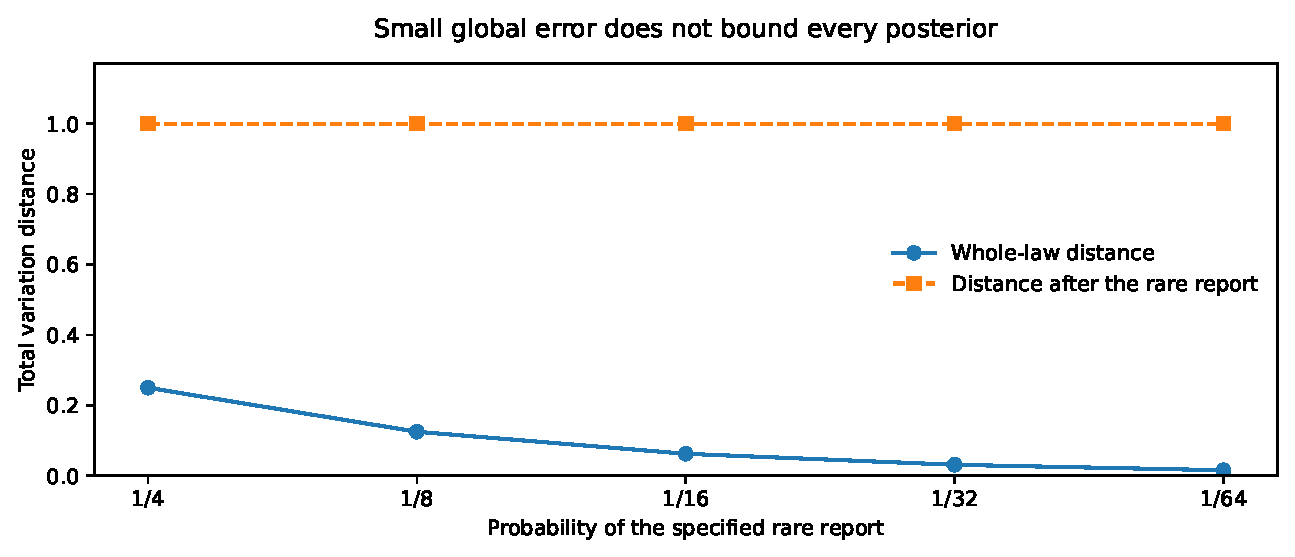
\includegraphics[width=.92\linewidth]{figures/rare_history.pdf}
\caption{In Counterexample~\ref{ce:rare-history}, shrinking the rare-event mass reduces whole-law error but leaves conditional error maximal. The points are exact specified probability laws, not sampled observations.}
\end{figure}

The bound compares one policy across two models, not independently optimized controllers. Chapter~\ref{ch:inquiry} supplies the uniform comparison needed for re-optimization. First, the next chapter asks what decisions and explanations the corrected record can justify.

\chapter{From corrected records to decisions and explanations}\label{ch:decision}
\question{The same record, model, and continuation must support the decision being certified.}
Correctness of a probability calculation is not a guarantee that a real process follows its likelihood model. Within the declared model, however, a small error in the retained distribution can support a precise decision bound. We state that bridge before introducing communication, so that an explanation has a definite object to preserve.

\section{One quantitative decision contract}
Let $p$ and $\widehat p$ be distributions on the same finite world set. For each world let $v_\omega$ be a response and $\widehat v_\omega$ its approximation in one metric space. Assume
\[
\TV(p,\widehat p)\le e,\qquad
\sup_\omega d(v_\omega,\widehat v_\omega)\le d_0.
\]
For each action $a$ in a finite nonempty set, let the loss $\ell(a,v)$ lie in $[0,1]$ and be $K$-Lipschitz in $v$. Define the model risks
\[
R(a)=\sum_\omega p(\omega)\ell(a,v_\omega),\qquad
\widehat R(a)=\sum_\omega\widehat p(\omega)\ell(a,\widehat v_\omega).
\]

\begin{theorem}[A decision bound for one actual approximation chain]\label{r:risk}
Put $\xi=\min\{1,e+Kd_0\}$. For every action, $|R(a)-\widehat R(a)|\le\xi$. If $\widehat a$ minimizes the approximate risk, then
\[
R(\widehat a)-\min_a R(a)\le\min\{1,2\xi\}.
\]
If the approximate gap between its unique minimizer and every alternative exceeds $2\xi$, that action is also the unique true model-risk minimizer.
\end{theorem}
\begin{proof}
Add and subtract $\sum_\omega p(\omega)\ell(a,\widehat v_\omega)$. The response term has absolute value at most $Kd_0$. The expectation of a function in $[0,1]$ changes by at most total variation, giving the other term at most $e$. Risks lie in $[0,1]$, so their difference is also at most one.

For a true minimizer $a_*$,
\[
R(\widehat a)\le\widehat R(\widehat a)+\xi
\le\widehat R(a_*)+\xi\le R(a_*)+2\xi.
\]
The loss range supplies the cap one. Finally, for any other $a$, subtract the two error bounds to obtain
$R(a)-R(\widehat a)\ge\widehat R(a)-\widehat R(\widehat a)-2\xi>0$.
\end{proof}
\source{[GA], ``A common quantitative grounding certificate''; [MU], ``A joint posterior and recipient decision certificate.'' This is a specialization to a common finite candidate set and bounded loss.}

The phrase ``model risk'' matters. The theorem cannot repair an omitted candidate, a false sensor convention, or an action outside the stated loss function. It also cannot combine a posterior bound from one history with a response bound from another. The record must bind the actual calculation and its premises.

For the noisy calibration example, use zero-one loss for selecting the target bit. Under $P$ and report one, choosing one has risk $1/4$, while choosing zero has risk $3/4$. An approximation with total variation at most $1/10$ and no response error preserves the unique decision because the gap $1/2$ exceeds $2/10$. Under $P'$ the correct decision reverses. A valid error bound around the wrong prior is not a substitute for retaining the correct association.

\section{An explanation belongs to a recipient}
An artifact is not an explanation merely because its producer can interpret it. Fix a finite case set $X$, a sender-access map $\alpha:X\to H$, and a finite artifact catalogue $\mathcal C$. Recipient $i$ has a background record $\beta_i(x)$, a demanded output $t_i(x)$, and a fixed bounded procedure $L_i$. A timeout, malformed artifact, wrong output, or budget overrun counts as failure.

Let $\mathcal C(x)$ be the artifacts that succeed for every recipient in case $x$. For an attained sender value $h$, put
\[
\mathcal C_h=\bigcap_{x:\alpha(x)=h}\mathcal C(x).
\]

\begin{theorem}[A common artifact for fixed recipients]\label{r:recipient}
A sender restricted to $\alpha(x)$ can provide one exact artifact for all recipients if and only if every $\mathcal C_h$ is nonempty. When feasible, the smallest possible number of distinct transmitted artifacts is
\[
\min\{|C|:C\subseteq\mathcal C,\ C\cap\mathcal C_h\ne\varnothing
\text{ for every attained }h\}.
\]
\end{theorem}
\begin{proof}
A sender seeing $h$ must choose the same artifact for all cases in that fibre. It must therefore select a member of $\mathcal C_h$, proving necessity. Choosing one member of each nonempty finite intersection gives a valid encoder. The image of any encoder intersects every $\mathcal C_h$. Conversely, any catalogue meeting all those sets supplies such an encoder by choosing from the intersections. Finite minimization gives the formula.
\end{proof}
\source{[MU], ``The fixed-recipient covering criterion.'' The earlier designed-decoder coloring criterion is not substituted for the installed-recipient problem.}

\begin{counterexample}[Individual acceptability is not a common message]\label{ce:message}
Two cases have the same sender record. In one, the sole acceptable artifact is $c_0$; in the other it is $c_1\ne c_0$. Each case has a valid explanation if its hidden identity is known. Their intersection is empty, so the sender cannot select a valid common explanation from its actual information.
\end{counterexample}

In the sensor, a sender observing $y$ can transmit one bit to a recipient holding $s$. The recipient's fixed XOR procedure returns $b=y\oplus s$. The sender need not know $b$: its message combines with the recipient's background.

A decoder that ignores this message fails where background alone cannot distinguish the target. More strings do not fix that procedure. Installed information, interpreter work, and message size are separate resources. The next chapter asks how the sender can acquire the needed information within one budget, counting every stored branch of the controller.

\chapter{One investigation, one resource budget}\label{ch:inquiry}
\question{A possible answer, an affordable observation, and a small program must belong to the same workflow.}
Let $X$ be a finite nonempty state space. It includes every origin tag, permission, background record, and history variable that affects the stated behavior. An experiment $e$ is allowed on a domain $D_e\subseteq X$, has a deterministic successor $f_e:D_e\to X$, a report $o_e:D_e\to O_e$, and a fixed nonnegative integer resource vector $c_e$.

A current support $V\ne\varnothing$ records possible states. The experiment is permitted only if $V\subseteq D_e$. After report $o$, the possible \emph{post-experiment} states are
\[
V_{e,o}=\{f_e(x):x\in V,\ o_e(x)=o\}.
\]
Only nonempty report branches are retained. If the target concerns a past value, that value must survive as an immutable tag. Resetting the current state is not recovering its history.

A terminal artifact $a$ is acceptable only if every fixed recipient succeeds in every state of $V$. Its worst-case terminal cost is $g_a(V)$, computed componentwise. A controller is a literal finite tree with one record per experiment or terminal node. Stored memory counts all branches, including those not visited in one execution.

\section{The complete finite frontier}
Let $\mathcal P_h(V)$ be the nondominated pairs $(v,m)$ of worst-case online resource vectors and stored-record counts attainable by successful trees with at most $h$ experiment steps. At depth zero the available pairs are
\[
\operatorname{Pareto}\{(g_a(V),1):a\text{ succeeds throughout }V\}.
\]
At greater depth retain those stops and, for each uniformly permitted experiment and one feasible child pair $(v_o,m_o)$ for every nonempty branch, form
\[
\left(c_e+\max_o v_o,\quad1+\sum_o m_o\right).
\]
A profile dominates another when it is no larger in every resource coordinate and strictly smaller in at least one. The maximum is componentwise. An impossible child contributes no tree; it is not a zero-cost branch.

\begin{theorem}[Exact joint feasibility for explicit controllers]\label{r:inquiry}
This recurrence gives exactly the nondominated resource profiles of successful depth-bounded controllers. Every retained pair has a concrete tree witness. A common online and storage budget is feasible if and only if it bounds one retained pair. Removing dominated child profiles does not change feasibility under any componentwise budget.
\end{theorem}
\begin{proof}
At zero depth the only possibilities are acceptable terminals, whose profiles are exactly the stated stops. At positive depth a successful tree either stops or begins with one uniformly allowed experiment. Every possible report needs a successful child on precisely $V_{e,o}$. By induction those children have profiles in the lower-depth attainable set. Worst-case online cost is the root cost plus their componentwise maximum. Complete tree storage is one plus the sum of all child records.

Conversely, combining any allowed root with a successful child for every report constructs a successful tree with that profile. This proves exact enumeration before pruning. Replacing a dominated child by a dominating one cannot increase either a coordinatewise maximum or a sum of record counts, and does not change its supported initial set. Thus Pareto pruning preserves every feasible budget and every retained profile has a witness.
\end{proof}
\source{[MU], ``A joint resource certificate for fixed recipients,'' and [SII], Theorem 6.2. The scalar-cost repair case is a specialization, not a different composition theorem.}

The recurrence can be expensive. It is a finite mathematical characterization, not an efficient general learner. It assumes its transition and acceptance tables. Their discovery and checking are preparation costs, not free consequences of the existence theorem.

\begin{counterexample}[Two separate optima do not form one controller]\label{ce:pareto}
There are four immutable cases, each requiring its own terminal answer. A direct observation of the case costs four units and gives a five-record tree including four terminals. Unit-cost equality tests can identify the case in at most three tests with seven records. Terminal answers have zero online cost in this particular example. The frontier is $(4,5)$ and $(3,7)$. The mixed budget $(3,5)$ is infeasible: an all-equality successful tree needs four leaves and at least seven records; any tree using the direct observation on a reachable path costs at least four.
\end{counterexample}

\begin{figure}[ht]
\centering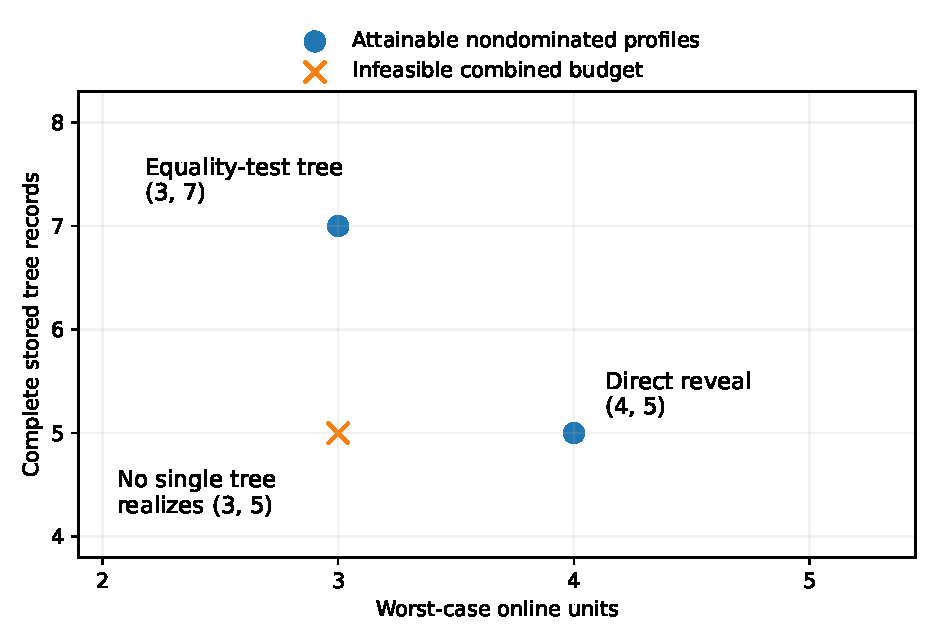
\includegraphics[width=.88\linewidth]{figures/joint_frontier.pdf}
\caption{The four-origin example has two nondominated profiles. Combining the lowest coordinate from each does not construct a feasible controller. Terminal answers have zero online cost in this example.}
\end{figure}

\section{When a checked candidate can end the search}
Consider $n\ge1$ immutable cases with total nondestructive binary unit-cost queries. Every unit-cost repair succeeds in exactly one case, and every case has a repair. A controller must succeed certainly in every case.

\begin{theorem}[A candidate attaining both lower bounds is optimal]\label{r:lowerbound}
Every successful controller has worst-case work at least $1+\lceil\log_2n\rceil$ and literal storage at least $2n-1$. A checked controller attaining both bounds and the requested horizon realizes the entire nondominated work/storage frontier.
\end{theorem}
\begin{proof}
Distinct cases cannot end at the same successful repair leaf, so at least $n$ leaves are reachable. A binary tree of query depth $d$ has at most $2^d$ leaves, giving $d\ge\lceil\log_2n\rceil$. The terminal repair adds one unit.

Let $l$ be the number of leaves and $i_1,i_2$ the counts of unary and binary internal nodes. Counting tree edges gives $i_1+2i_2=i_1+i_2+l-1$, hence $i_2=l-1$. Total records are $2l-1+i_1\ge2n-1$. A successful candidate at both coordinatewise lower bounds dominates every other attainable cost profile. Its validity and horizon check make it an actual member of the frontier, leaving that pair as the whole nondominated frontier.
\end{proof}
\source{[SII], Theorem 11.1. The assumptions exclude destructive resets and repairs that succeed on several cases.}

For eight possible defective cells, equality-first diagnosis requires seven queries in the worst case, while three coordinate-bit queries identify the cell. Including repair gives costs eight and four, respectively. Both literal trees have fifteen records. Faster execution has not eliminated the cost of storing the procedure.

This eight-cell example is separate from the eight-world sensor. The sensor has only four action-relevant $(b,s)$ pairs and an irrelevant nuisance coordinate. Confusing hidden-world cardinality with the number of required repair distinctions would import a false lower bound.


\section{Expected-cost inquiry uses the report probabilities}
The preceding frontier certifies worst-case execution and complete tree storage for deterministic observations. A noisy report requires a different optimization. Expected cost weights each future branch by its probability. A low expectation is not a hard execution budget, and neither replaces the cost of storing the whole controller.

Use the finite instrument of Theorem~\ref{r:instrument}, with fine belief $p$ and coarse belief $q=Cp$. At $q$, a finite set of experiments $A(q)$ is permitted, and a nonempty finite set of terminal decisions $D(q)$ is available. These catalogues must be identical for every fine belief with the same $q$. Stopping with decision $d$ has loss $\ell_d(\pi(x))$ in fine state $x$, so its conditional risk is $\langle q,\ell_d\rangle$. An experiment has a finite nonnegative charge $c_a(q)$, identical on the fine and coarse side. All history variables affecting permissions, charges, or targets must be included in the declared state.

Let $J_h(p)$ be the least expected charge plus terminal loss attainable using at most $h$ further experiments, with terminal decisions permitted at any step. It is defined by finite observation trees, not by a hidden-state controller. Its coarse recurrence is
\begin{align*}
 \bar J_0(q)&=\min_{d\in D(q)}\langle q,\ell_d\rangle,\\
 \mathcal Q_h(q,a)&=c_a(q)+\sum_{o:\bar z_{a,o}(q)>0}
       \bar z_{a,o}(q)\bar J_{h-1}\bigl(\bar\Psi_{a,o}(q)\bigr),\\
 \bar J_h(q)&=\min\left\{\bar J_0(q),\ \min_{a\in A(q)}\mathcal Q_h(q,a)\right\}.
\end{align*}
An empty experiment catalogue leaves only stopping. Impossible reports do not receive invented posteriors.

\begin{theorem}[The same compressed belief supports the same inquiry]\label{r:belief-planning}
Under the exact instrument quotient and the common loss, charge, and catalogue assumptions above,
\[
 J_h(p)=\bar J_h(Cp)\quad\text{for every prior and every finite }h.
\]
Every first-action value and optimal first-action set agrees. A minimizing coarse-belief policy produces a fine-model optimal history-based policy, including its stopping decision. Finite minimizing trees exist. The result supplies neither an efficient synthesis algorithm nor a worst-case storage or resource guarantee.
\end{theorem}
\begin{proof}
At zero horizon the terminal risks agree by fibrewise summation. Suppose the equality holds at $h-1$. For any permitted first experiment, Theorem~\ref{r:instrument} gives the same probability of each report and the same coarse posterior on every positive branch. The induction hypothesis gives equal optimal continuation costs on each such branch. The first charge agrees, so the entire action value agrees. Stopping has the same value as well. Taking the minimum over the identical catalogues proves both value equality and equality of minimizing first choices.

Choose one minimizing first choice and attach minimizing lower-horizon trees to its finitely many positive branches. If the choice is terminal, no child is required. Induction constructs a finite tree attaining the value. The same induction bounds every other admissible tree below by that minimum. An observed history initializes the same coarse belief in the fine execution, so selecting from that belief realizes the coarse policy without observing the fine hidden state.
\end{proof}
\source{The finite backup and projected-law proof mechanisms of [AVOC], Theorems 4.5 and 9.2, applied here to the belief transition supplied by Theorem~\ref{r:instrument}. This is a prose composition, not a newly kernel-checked instance of AVOC. The established partially observed planning context is [KLC].}

\begin{counterexample}[A correct probability quotient can hide a forbidden action]\label{ce:permission-loss}
Two fine states share all report and transition probabilities and are given the same coarse label. A terminal repair is permitted in one state but forbidden in the other. The instrument quotient is valid, but a coarse interface that offers the repair in both states is not. Exact belief and value formulas do not repair a missing permission distinction. The catalogues must factor through the retained state, or the state must be refined.
\end{counterexample}

\section{The sensor chooses when another calibration is worth its cost}
Return to the sensor after display $y=0$. Conditional on that display, assign equal probability to $(b,s)=(0,0)$ and $(1,1)$, with any nuisance distribution inside each pair. Only noisy calibration and terminal bit selection are offered in this example. A calibration reports $s$ correctly with probability $3/4$, with fresh conditionally independent noise and no change to the hidden world. It costs $1/20$ in the same stated loss units as a wrong terminal choice, whose loss is one. A correct terminal choice has loss zero.

The retained belief on the four $(b,s)$ pairs is an exact quotient of the eight-world belief. Its two diagonal masses initially equal $1/2$. After one calibration the favored target has probability $3/4$. A second matching report raises that probability to $9/10$, while conflicting reports restore $1/2$.

\begin{center}\begin{tabular}{@{}>{\raggedright\arraybackslash}p{.16\linewidth}>{\raggedright\arraybackslash}p{.24\linewidth}>{\raggedright\arraybackslash}p{.54\linewidth}@{}}\toprule
Report limit & Optimal expected cost & An optimal initial choice\\\midrule
0 & $1/2$ & Stop and select either bit.\\
1 & $3/10$ & Calibrate once, then select.\\
2 & $3/10$ & Calibrate once, then stop.\\
3 & $11/40$ & Calibrate, then use an adaptive continuation.\\\bottomrule\end{tabular}\end{center}

\begin{figure}[H]
\centering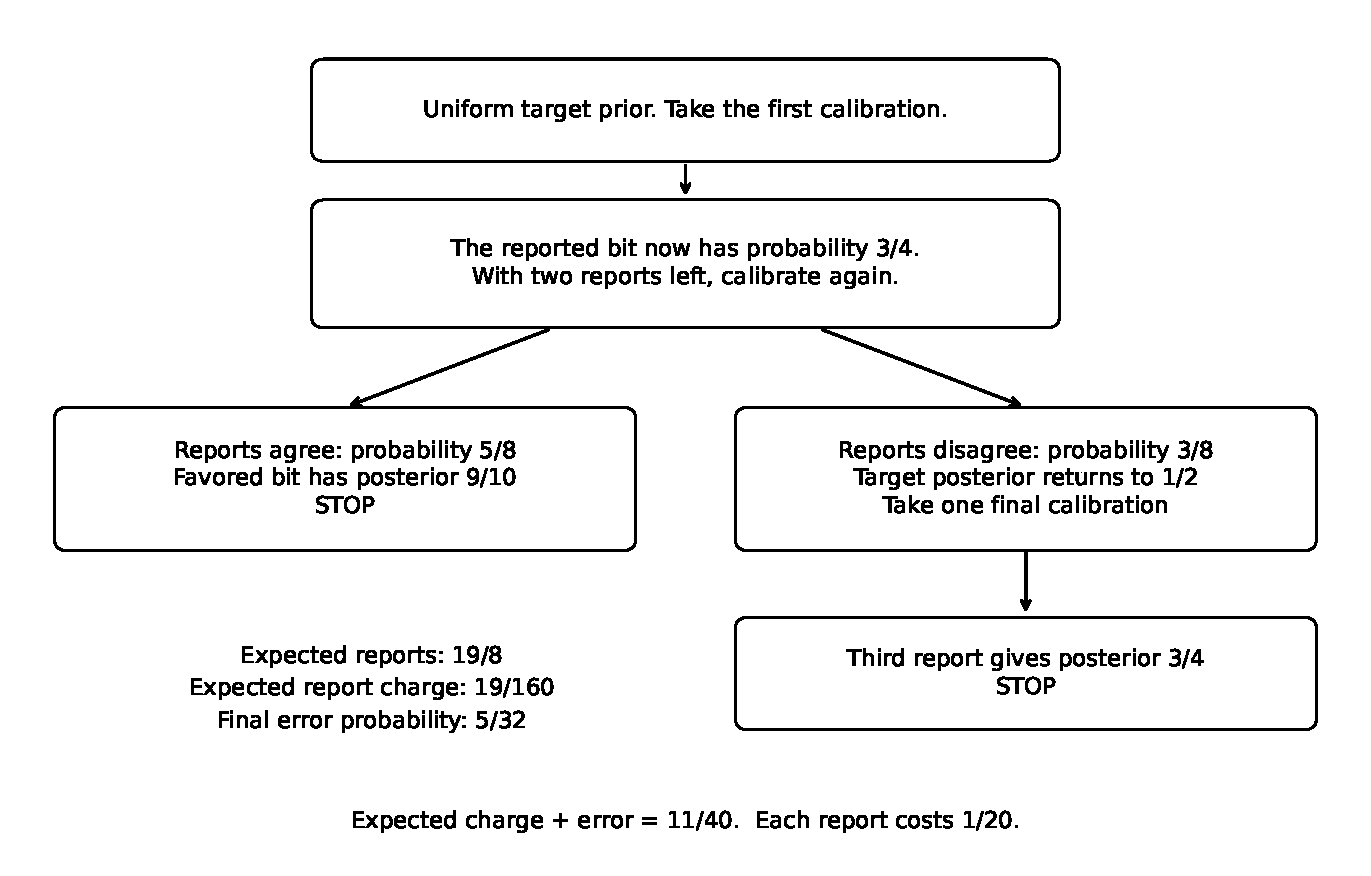
\includegraphics[width=.94\linewidth]{figures/calibration_policy.pdf}
\caption{An optimal three-report policy in the unchanged eight-world sensor with the explicitly added noisy calibration channel. All masses and costs are exact. The diagram groups sign-symmetric report histories, not distinct hidden states supplied to the agent.}
\end{figure}

With three reports available, the optimal policy takes a second report after the first. If the first two agree, it stops. If they disagree, it takes the third. The disagreement probability is $3/8$. Thus the expected report count is $2+3/8=19/8$, the expected charge is $19/160$, and the error probability is $5/32$. The total is $19/160+5/32=11/40$.

A horizon of two does not improve on one in this model: after the first result, paying for one additional report does not lower expected classification error enough to recover its charge. A horizon of three creates the option to investigate only the unresolved branch. The value comes from one contingent policy, not from separately optimal answers selected after the hidden bit is disclosed.



The two-valued predictive display state from Chapter 1 is too coarse for this inquiry. The four-pair probability record supports every calibration update and decision while still discarding the nuisance bit. This is the promised chain from evidence to representation to a useful experiment choice.

\section{An approximate model supports a different, quantitative claim}
Exact policy transport and approximate planning must not share one unqualified guarantee. Fix a finite horizon $H$ and one finite class $\mathfrak P$ of admitted action/report trees, shared by the true and approximate models. The complete loss of a tree is the same function of its coarse-state and action/report path in both models, taking values in $[0,B]$. For example, a terminal loss in $[0,1]$ and at most $H$ charges bounded by $c_{\max}$ give $B=1+Hc_{\max}$.

Assume Theorem~\ref{r:history-bound}'s bound $d_H$ holds uniformly over every tree in that class. An early stop is padded by a common absorbing terminal step for the history comparison. State-dependent charges are permitted when included in the same coarse-path loss. A model-dependent posterior score used as an uncharged surrogate loss would be a different problem.

\begin{proposition}[Uniform model error controls a changed policy]\label{r:policy-error}
Let $J(\pi)$ and $\widetilde J(\pi)$ be a tree's expected losses in the true and approximate models. Then
\[
 |J(\pi)-\widetilde J(\pi)|\le Bd_H\quad(\pi\in\mathfrak P).
\]
If $\widetilde\pi$ minimizes the approximate loss and $\pi_*$ minimizes the true loss over this same class, then
\[
 J(\widetilde\pi)-J(\pi_*)\le\min\{B,2Bd_H\}.
\]
These conclusions do not certify a zero-risk constraint or preservation of admissibility outside the common class.
\end{proposition}
\begin{proof}
The expectation of a function in $[0,B]$ changes by at most $B$ times total variation. Apply the common-policy history bound separately to each fixed tree, proving the first assertion uniformly. Now
\[
 J(\widetilde\pi)\le\widetilde J(\widetilde\pi)+Bd_H
 \le\widetilde J(\pi_*)+Bd_H\le J(\pi_*)+2Bd_H.
\]
The range of loss gives the cap $B$. The proof compares each tree with itself across the models before using the optimality inequality. It never applies a same-policy bound directly to two different controllers. A bad event assigned probability zero in one model can have small positive probability in the other, so an average bound supplies no sure-feasibility conclusion.
\end{proof}
\source{Direct combination of the newly admitted whole-history bound with the selection argument already used in Theorem~\ref{r:risk}; [AVOC], Sections 8--10, provide the source context for guarded planning and model-error value bounds. This finite fixed-policy-class formulation is stated and proved in full here.}

With true calibration accuracy $37/50$ and planning accuracy $3/4$, the one-step defect is $1/100$. For $H=3$ and $B=23/20$, the uniform regret bound is $69/1000$. Exact observed performance is reported separately, not substituted for this guarantee. Expected-risk and hard-budget checks remain distinct. Next we study changes to the compiler producing the inquiry.

\chapter{Improving discovery without changing its meaning}\label{ch:discovery}
\question{Removing redundant work is an improvement only when the removed work could not change the justified result.}
Let $\mathcal G=(p_0,\ldots,p_{N-1})$ be a finite ordered grammar of pure, total candidate programs. Let $D$ be a finite context set and $t:D\to Y$ a fixed labeling. A teacher either accepts a candidate that agrees everywhere or returns a context where it disagrees. The teacher's work is part of the development account.

\section{Finite counterexample-guided acquisition}
The learner retains every returned counterexample. It proposes the earliest candidate consistent with all retained examples, or reports exhaustion of the grammar when none remains.

\begin{proposition}[What finite counterexamples establish]\label{r:cegis}
The learner never submits the same rejected candidate twice. Within at most $N$ teacher calls, it returns the earliest globally correct candidate in the declared grammar or exhausts that grammar. A timeout before this process finishes is neither acceptance nor exhaustion.
\end{proposition}
\begin{proof}
Each counterexample refutes the submitted program and remains a constraint forever. That program cannot be submitted again. A globally correct candidate never violates a truthful counterexample. With only $N$ candidates, either an accepted one is found or all are ruled out. If the accepted candidate were preceded by a globally correct candidate, that earlier candidate would still be consistent and would have been selected first. This proves the ordering claim. Interruption changes none of these logical implications and cannot supply a completed search result.
\end{proof}
\source{[SII], Theorem 15.1. This is finite exact synthesis in a supplied language, not a statistical generalization guarantee.}

Agreement on $D$ is not validity outside $D$. That distinction is especially important when a candidate is used to prune future searches. A wrong proposal can be rejected by a final checker. A wrong pruning rule may remove the only candidate the checker ought to see.

\section{A learned search representation can preserve the exact investigation}
Suppose a deterministic normalizing map $n$ is sound in the following direction:
\[
n(p)=n(q)\ \Longrightarrow\ p(z)=q(z)\quad\text{for every admitted context }z.
\]
The map need not detect every semantic equivalence or produce a mathematically canonical normal form. Each successful contextual rewrite must be justified under the actual pure, total semantics. Keep the earliest original AST for every attained normal form, not a replacement AST with an uncharged new interpreter.

\begin{theorem}[Ordered semantic compression preserves the teacher trace]\label{r:ordered}
Assume all counterexamples are retained, candidate and example orders are fixed, and the teacher is deterministic and extensional, returning the first disagreement in a fixed context order. Searching only the earliest representatives yields exactly the same submitted ASTs, counterexamples, and final acceptance or grammar exhaustion as the original learner. With the same AST interpreter it uses no more retained-example evaluations. Preparation, dispatch, and stored-index costs are separate.
\end{theorem}
\begin{proof}
A removed expression has an earlier representative with the same values on every admitted context. If that representative was accepted, the original search ended before reaching the removed expression. Otherwise an already retained example refuted the representative, either during a consistency test or from the teacher. Persistence of examples means that the same example refutes the later equivalent expression. The original learner therefore never submits that removed expression to the teacher.

Deleting only those unsuccessful consistency tests preserves the next submitted AST. A deterministic teacher then returns the same counterexample or acceptance. Induction over submissions proves equality of the complete trace, including exhaustion. Every deleted evaluation has nonnegative cost in the named evaluation count. The argument makes no claim that constructing or consulting the representative index is free.
\end{proof}
\source{[SII], Theorems 21.1 and 21.2. Sound equational replacement is the premise; empirical agreement on a few probe points does not supply it.}

\begin{counterexample}[A probe-equivalent equation is not a general identity]\label{ce:probe}
The expressions $\max(x,1)$ and $x$ agree for probes $x\in\{1,2,3\}$. At zero they differ. Grouping them by those probe values alone can remove a needed candidate. The identity $\max(x,0)=x$ is valid over nonnegative integers, but not over all integers. The semantic domain is part of the equation's certificate.
\end{counterexample}

The retained object may therefore improve later search without containing its answers. This is the precise process-level role of a checked equation library. The grammar, primitive semantics, teacher, and proof rules can still be supplied. Their presence must remain visible instead of being redescribed as discoveries.

\section{A reusable rule for stopping an unpromising read}
A diagnostic compiler inspects a binary query on $m$ immutable cases. In the prefix already read, $a$ cases give zero and $b$ give one. Each child is allowed at most $C$ cases because the remaining binary depth has that leaf capacity. Assume integers
\[
C\ge1,\quad 2\le m\le2C,\quad a,b\ge0,\quad a+b\le m.
\]

\begin{proposition}[A sound prefix exclusion]\label{r:prefix}
The unread reports can be completed with both final branch counts at most $C$ if and only if $\max(a,b)\le C$. A scan may therefore stop when one count first exceeds $C$. In a fixed ordered depth-first compiler with identical scope, terminal, and fallback rules, replacing full root scans by this early rejection preserves the first returned tree or the completed depth-bounded failure result.
\end{proposition}
\begin{proof}
Counts only increase, so an overfull child cannot be rescued. Otherwise the two remaining capacities are $C-a$ and $C-b$, both nonnegative. Their sum $2C-a-b$ is at least the number $m-a-b$ of unread rows. Distributing the unread cases between those capacities gives a feasible completion.

Every root rejected early would also be rejected after its full scan. A root not rejected early is read completely and produces the same ordered child supports. Induction on the finite remaining depth therefore yields identical recursive searches, backtracking, and first completion. The same failure condition invokes the same fallback. The skipped rows are only suffixes whose contents could not change rejection. A resource timeout is excluded from the completed-failure claim.
\end{proof}
\source{[SII], Proposition 16.1 and Theorem 16.3. The conclusion concerns capacity feasibility, not the existence of a completing query in the installed language.}

For $C=4$, a fifth zero already closes a root. Reading more rows cannot reduce that branch. By contrast, a four-versus-four split merely survives this necessary test. If no remaining query distinguishes either child, the root still fails.

\begin{counterexample}[A changed repair defeats the old premise]\label{ce:universal}
Four cases previously required four different repairs. Admit one new repair successful in all four. No identifying query is now needed. The old singleton-leaf lower bound and its pruning interpretation are not applicable. The correct response is to recheck the repair scope, not to preserve an obsolete optimization because it once passed.
\end{counterexample}

\section*{What is now available}
The resulting method is semantically justified only under its premises. We must still determine whether it saves total resources, and which proof records remain usable when a later revision changes those premises. Both questions belong to the next chapter rather than being inferred from a successful synthesis.

\chapter{What remains valid after a revision}\label{ch:revision}
\question{A mathematical proof can remain true while no longer applying to the installed system.}
A certificate for ordinary integer addition is not a certificate for an operation with the same printed name and a different implementation. A grammar quotient depends on the grammar order. A comparison depends on the actual controller and the prices used to value its events. These are distinct dependencies.

\section{Reuse follows semantic dependencies}
Let an artifact state be $a=(a_1,\ldots,a_d)$. A finite directed acyclic graph represents claimed guarantees. For vertex $v$, let $D_v$ be its direct artifact dependencies and let $\operatorname{pa}(v)$ be its parent guarantees. The declaration is semantically complete if the meaning of its claim and local verification rule is determined by those components and parent claims. External assumptions are included explicitly as premises.

After changing $a$ to $a'$, mark a vertex stale when a direct input changes and propagate staleness to all descendants. Call the resulting set $\Delta$.

\begin{theorem}[Selective reuse with complete dependencies]\label{r:dependencies}
Assume the graph is finite and acyclic, direct dependencies are semantically complete, local rules are sound, and the applicable external premises hold. Assume also that every old witness established its old claim before the revision. Old witnesses still establish every claim outside $\Delta$. Re-establishing affected claims in topological order, using revised values and established parents, restores the corresponding revised claims. Without an affected parent's re-establishment, this reuse rule supplies no justification for its dependent claim.
\end{theorem}
\begin{proof}
A vertex outside $\Delta$ has unchanged direct values and no stale parent. In topological order, induction shows that every parent retains its meaning and proof. Completeness of the dependency declaration leaves the local argument applicable. For a stale vertex, once its revised parents are established, soundness of the newly checked local rule gives the revised conclusion. A second topological induction proves restoration. An unchecked parent leaves a missing premise, so the rule alone cannot justify a dependent conclusion. This is not a proof that the conclusion is false.
\end{proof}
\source{[SII], Theorem 24.1. It is a theorem about a declared complete dependency graph, not a method that infers complete dependencies from arbitrary programs.}

\begin{counterexample}[A missing dependency defeats a perfect replay]\label{ce:dependency}
A stored claim is $u=v$, initially with both values zero. Its registry records only $u$. Change $v$ to one. A flawless comparison with the recorded $u$ still passes, while the claim is false. A hash or replay cannot recover the premise the registry omitted.
\end{counterexample}

Adding the universal repair from the preceding chapter changes a successful-repair set. It invalidates a cardinality certificate and any dependent performance statement. It need not invalidate an arithmetic equation used elsewhere. A new valid repair also does not inherit the old controller's speed comparison. Rechecking can legitimately conclude that the new route is slower, cheaper, or incomparable under the stated resources.

\begin{figure}[ht]
\centering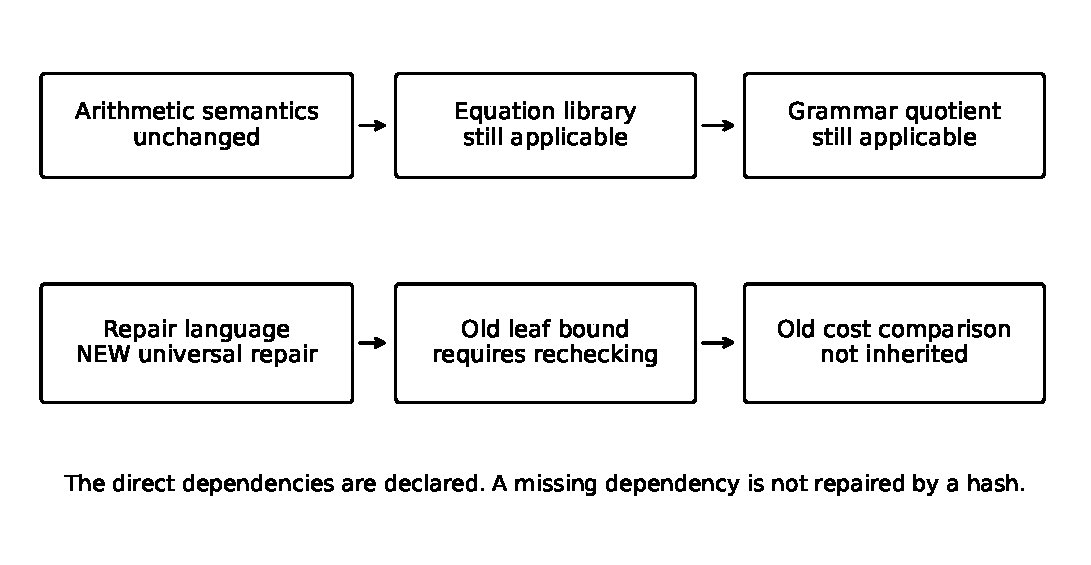
\includegraphics[width=\linewidth]{figures/revision_scope.pdf}
\caption{A change to the repair language affects the diagnostic justification but need not change arithmetic semantics. The depicted graph is a declared example, not an automatically discovered dependency registry.}
\end{figure}

\section{Semantic improvement and resource improvement are separate}
Fix named additive event types. Let $K\ge0$ be an extra preparation vector, let $s_i$ be the old-minus-new per-use vector for workload type $i$, and let $n_i$ count its uses. The net event difference is
\[
\Delta=\sum_i n_i s_i-K.
\]
A nonnegative price vector $w$ converts these events into one declared additive measure. Storage capacity, peak memory, and elapsed time need their own models unless a justified conversion is specified.

\begin{proposition}[Which gains survive every admitted price?]\label{r:prices}
The saving $w\cdot\Delta$ is nonnegative for every nonnegative price vector if and only if every coordinate of $\Delta$ is nonnegative. If prices lie in the convex hull of a finite nonempty set $W$, their minimum saving equals $\min_{w\in W}w\cdot\Delta$.
\end{proposition}
\begin{proof}
A componentwise nonnegative vector has nonnegative inner product with every nonnegative vector. If coordinate $j$ is negative, assigning price one only to that coordinate gives a negative result. This proves the first assertion. A point in the stated convex hull is a convex combination of its listed prices, so its saving is the same convex combination of their savings. It cannot be smaller than the minimum listed value, and a listed minimizer attains that value.
\end{proof}
\source{[SII], Proposition 25.1. No hardware performance law follows from this additive accounting identity.}

For the source's checked weighted-search comparison, the event difference is $(1552,1552,-1868)$ in reads, rational additions, and comparisons. Equal prices give $1236$ saved units. Prices $(1,0,1)$ give a loss of $316$. Both conclusions concern the same valid controller. The main text uses this as a transparently rechecked source calculation, not as a new measured timing result.

\section{Evidence across an adaptive sequence}
A procedure that searches many candidates can select a favorable error in its evaluator. The right statement must therefore condition on the information that produced the candidate, not merely repeat a marginal error bound for a candidate fixed in advance.

\begin{proposition}[A conditional error budget for a lineage]\label{r:lineage}
Let $\mathcal H_{j-1}$ contain the information available before attempt $j$. Suppose the event $A_j$ of accepting a false claim satisfies
\[
\Pr(A_j\mid\mathcal H_{j-1})\le\delta_j\quad\text{almost surely},
\qquad\sum_{j\ge1}\delta_j\le\delta,
\]
for deterministic nonnegative $\delta_j$. Then the probability of ever accepting any false claim is at most $\delta$, even when candidates and the stopping time depend on earlier history.
\end{proposition}
\begin{proof}
Taking expectations gives $\Pr(A_j)\le\delta_j$. A union bound gives the result for every finite set of attempts. The finite unions increase to the event of any false acceptance, so continuity of probability gives the infinite statement. Stopping removes attempted events and cannot enlarge their union.
\end{proof}
\source{[SII], Proposition 26.1. The mathematical input is conditional validity of each actual attempt. A numerical error schedule alone does not establish that premise.}

This proposition is not an empirical result about a population of agents. It explains what evidence would need to remain valid when an evaluator is used adaptively. Deterministic exact checks in this book are not treated as statistical samples and are not assigned confidence intervals through this formula.

\section*{What is now available}
A revision can preserve its meaning, identify stale obligations, and state its resource advantage under explicit prices. None of this yet determines what several participants can know together or which authority they should exercise. The final technical chapter keeps information sharing and institutional permissions separate while applying the same preservation discipline.

\chapter{Shared work and maintained obligations}\label{ch:shared}
\question{Joint information can support a task without creating a single decision maker.}
One agent may have a display record and another a calibration record. Neither need know the physical target bit alone. Together their records can determine it. This is an informational relation before it is any claim about collective agency.

\section{What several accessible records can reconstruct}
Let $V$ be a finite-dimensional vector space over a field. Participant $i$ has a linear record $A_i v$. Stack the records into $Av=(A_1v,\ldots,A_mv)$, and let $Qv$ be the protected linear target.

\begin{proposition}[Target-relative joint reconstruction]\label{r:reconstruction}
There is a linear decoder $D$ with $Q=DA$ if and only if $\ker A\subseteq\ker Q$. Full-state reconstruction is possible exactly when $A$ is injective. The intersection identity $\ker A=\bigcap_i\ker A_i$ determines which ambiguities sharing removes.
\end{proposition}
\begin{proof}
If $Q=DA$, a vector annihilated by $A$ is also annihilated by $Q$. Conversely, define $D(Av)=Qv$ on $\im A$. If $Av=Aw$, then $v-w\in\ker A\subseteq\ker Q$, so this definition is independent of the representative. It is linear and extends to the full record space by extending a basis. For $Q=I_V$ the kernel condition is injectivity. A stacked record vanishes exactly when each component record vanishes, giving the intersection identity.
\end{proof}
\source{Target-relative specialization of the reconstruction and factorization machinery in Sufficient Resolution [SR] and Stratified Relational Workspace Theory [SRWT]. The proof here does not import their complete noise, dynamics, or identity theories.}

Over $\mathbb F_2$, Agent A observes $A_A(b,s)=b+s$ and Agent B observes $A_B(b,s)=s$. The joint matrix is invertible. Either agent alone lacks a direction needed to recover $b$. The nuisance bit may remain unknown because the target map ignores it.

The theorem concerns accessible records. It does not send them. A communication protocol, truthful interpretation, permitted disclosure, and the recipient's executable decoder remain separate requirements. Chapter~\ref{ch:decision} states the corresponding fixed-recipient criterion.

\section{Permissions are part of an operational state}
Now let a finite institutional state $x$ have a protected label $\ell(x)$, an enabled-action set $D(x)$ within a fixed finite alphabet, and a deterministic successor $F(x,a)$ for enabled actions. Labels may include resource balances, outstanding obligations, and offices, but need not retain every historical byte.

\begin{theorem}[A quotient that preserves legal operations]\label{r:governance}
For a surjection $\pi:X\to Z$, quotient labels, enabled sets, and successors satisfying
\[
\ell=\bar\ell\pi,\qquad D=\bar D\pi,\qquad
\pi F(x,a)=\bar F(\pi x,a)
\]
exist exactly when equal fibres have equal labels, equal enabled sets, and equal projected successors for every enabled action. The quotient data are unique and preserve every legal finite action and label sequence.
\end{theorem}
\begin{proof}
Factoring each quantity proves necessity. For sufficiency choose a representative of each fibre to define its label, enabled set, and successor. The three equalities make those definitions independent of the representative. Surjectivity gives uniqueness. Equal enabled sets admit the same first action, and successor equality preserves membership in one fibre. Induction on the sequence length preserves legality and all labels.
\end{proof}
\source{[MS], ``Exact governance quotient.'' This extends the deterministic behavioral construction by explicitly protecting action availability. It does not derive moral or external legal authority from the state description.}

A summary that preserves only the next sensor response can merge states in which a repair is authorized with states in which it is forbidden. It may remain a good predictor while becoming an invalid action interface. The necessary correction is to preserve the enabled-set distinction, not merely to attach a reassuring name to the old code.

\section{Continuing should not erase the ability to finish}
Use a finite \emph{observed} configuration space $Z$. Under partial observation, the configurations would instead have to be justified public possibility states. At $z$ there are finite catalogues of running actions and ending actions, each with a nonempty successor set. A declared safe set is $S$, and an ending target is $G\subseteq S$. A safe hold action is available at $G$.

A stop command is assumed authentic and observable before the next action is selected. Its delivery and authentication are premises, not consequences of the following fixed-point calculation. Define
\begin{align*}
T_0&=G,\\
T_{k+1}&=T_k\cup\{z\in S:\exists a\in A_{\rm end}(z),\ \operatorname{Post}(z,a)\subseteq T_k\}.
\end{align*}
Let $T_*$ be the stable set. Then define
\[
L_0=T_*,\qquad
L_{k+1}=\{z\in L_k:\exists a\in A_{\rm run}(z),\ \operatorname{Post}(z,a)\subseteq L_k\},
\]
and let $L_*$ be its stable value. Both sequences stabilize because $Z$ is finite.

\begin{theorem}[Safe continuation that retains an ending strategy]\label{r:ending}
A starting configuration belongs to $L_*$ exactly when one policy can run safely indefinitely without a stop command and, after a stop command at any decision epoch, reach $G$ on every possible successor path using only the admitted ending actions. Before the command a policy preserving $L_*$ suffices. After the command it can reach $G$ within the first-entry rank of the current state in the $T_k$ sequence.
\end{theorem}
\begin{proof}
Induction shows that membership in $T_k$ is equivalent to an ending-only policy reaching $G$ within $k$ transitions while staying safe. The chosen action moves every successor to a smaller rank. Outside $T_*$, every ending action has a successor outside $T_*$ or outside safety. Choosing such a successor at every step defeats any purported surely safe ending. Thus $T_*$ is exactly the sure-ending region.

At $L_*$ a running action keeps every successor inside $L_*$. Repeatedly using such actions is safe and retains membership in $T_*$. A command can therefore switch to the decreasing-rank ending policy at any epoch.

Conversely, if a policy has the stated guarantee, every pre-command reachable configuration must admit an ending immediately and hence lie in $T_*$. For any finite number of further running steps, it must keep all paths in that set. Induction in the decreasing construction places the initial state in every $L_k$, hence in $L_*$. No action is chosen after secretly observing its successor.
\end{proof}
\source{Fully observed finite specialization of [MS], ``Continued operation with an available authorized ending.'' The more general public-possibility construction is not silently assumed in this version.}

\begin{counterexample}[Safe inactivity without an ending]\label{ce:ending}
A state $z$ has a safe idle self-loop and no ending action reaching $G$. It is safe forever but outside $T_*$. In a second state $u$, an ending is available, while the only running action spends its reserved resource and moves to $z$. Then $u$ belongs to $T_*$ but not $L_*$. Being able to stop now does not establish that ordinary operation preserves that ability.
\end{counterexample}

These results do not establish society formation, strategic compliance, or a just constitution. They establish information, action, and continuation properties of a specified finite institution. Their place at the end of the book is earned by the preceding account of accessible evidence, common artifacts, feasible controllers, and dependency-preserving revision.

\chapter{One continuous chain, with no hidden promotion}\label{ch:close}
The sensor story can now be followed without changing the meaning of a record midway through the argument.

Begin with eight candidate worlds $(b,s,n)$. The agent's initial display $y$ determines its two-state predictive class under flips, but not the physical target bit. The first chapter proves both claims. The second gives the operator on the retained class and the coordinate map that becomes usable after calibration. Neither requires the nuisance bit.

When display and calibration observations arrive, candidate sets are filtered. The third chapter proves why the joint association must be retained, and why sixteen occupancy states suffice for the exact partition-evidence contract. Under a separately declared noisy calibration, four probability masses replace the occupancy bits. The same numerical posterior cannot be inferred from separate marginals. The enlarged chapter now requires a joint report/next-state law, not only correct separate marginals. Its finite refinement makes the required distinctions explicit, and its history bound states the separate price of conditioning on a rare report.

The fourth chapter places that posterior and any response approximation under one loss function. It also specifies what a recipient can decode from a message and its prior record. The fifth asks whether the sender can acquire the missing observation and transmit a successful artifact within a single online and stored-controller budget. The complete tree is counted even if an execution visits only one path. A separate noisy-calibration calculation then uses the exact same retained belief to select a finite expected-cost inquiry. Uniform whole-history error supports a quantitative policy comparison, but not an automatic hard-budget or zero-risk guarantee.

The sixth chapter then changes the discovery procedure rather than the hidden world. Checked equations can remove equivalent candidates while preserving every teacher proposal and counterexample. A separately justified capacity rule can stop reading an impossible diagnostic root. Neither step invents the primitive grammar, the teacher, or the theorem used to authorize pruning.

The seventh chapter binds those uses to their premises. Adding a universal repair changes the required diagnostic distinctions. The old lower bound becomes inapplicable; arithmetic identities need not. A fresh cost comparison may find a saving or a loss. The eighth chapter finally combines different participants' records and asks what actions they are entitled to perform under their declared institutional state. Safe indefinite operation and preservation of an authorized ending are checked separately.

\section{A worked end-to-end record}
Take the actual illustrative world $(b,s,n)=(0,1,1)$. The complete protocol begins with all eight worlds possible:
\begin{center}\begin{tabular}{p{0.25\linewidth}p{0.27\linewidth}p{0.35\linewidth}}\toprule
Event & Remaining worlds & What is justified\\\midrule
Before observation & All eight & No physical target identified.\\
Display $y=1$ & Four worlds & Predict every later display flip.\\
Calibration $s=1$ & Two worlds differing only in $n$ & Physical target $b=0$.\\
Send $y$ to a recipient holding $s$ & Same two worlds & Recipient computes $b=0$ through its fixed XOR decoder.\\
Commit the authorized target action & As declared by its effect & One action justified across the current support.\\
Record the fulfilled obligation & Includes the action's receipt & Continuation or ending can refer to the actual completed act.\\\bottomrule\end{tabular}\end{center}

The witness does not claim to have discovered its sensor semantics. Its exact checking confirms the stated scenario. Another physical process requires its own evidence. A failed receipt, an untrusted calibration, or an altered action effect changes the guarantee rather than being averaged away as a small numerical error.

\section{Why the core is narrower than the archive}
This book does not append the old Neuralese experimental history, proposed PRISM architecture, full SRIC lineage, or every formal guide. Their presence would make the reader repeatedly switch between a proved conditional statement, a proposed mechanism, a historical execution, and an implementation plan. Those are useful source objects, but they are not one continuous proof.

Selected source results are restated and proved where they carry the argument. Selected stochastic-value arguments from AVOC enter through complete prose proofs and explicitly matched finite models. Their selected formal counterparts are identified in the companion; this does not import AVOC's complete formal development or the specialist Certified Bayesian Inference construction. Source pedigree alone supplies no blanket assurance for the wider source corpus.

Nor is a source excluded merely because it contains open questions. Its proved results can be considered individually. A claim enters when its exact form, dependencies, and evidence have been reviewed at the level promised for this edition. This is a stricter and more useful rule than treating every page of a final-named document as equally checked.

\section{The result of the compilation}
The core establishes a connected conditional account of accessible state, meaningful operations, corrective memory, usable explanations, bounded investigations, justified search changes, and maintained obligations. The arguments share several elementary constructions, but each use preserves its distinct type and hypotheses.

No theorem here turns a semantic interface into a trained neural model, a finite investigation into general intelligence, a shared record into a collective subject, or an invariant into legitimate external authority. The mathematical contribution is the explicit chain and the failures that break it. Those failures can be investigated without changing the standard of proof or requiring a large implementation campaign.

\backmatter
\chapter{Formal correspondence}
The selected finite reasoning core has formal counterparts for all twenty-seven source results. The correspondence covers the chain developed in the eight mathematical chapters: accessible evidence, representation and probability, correction memory, decisions and explanations, bounded inquiry, search, revision, and maintained obligations.

For evidence consisting exactly of unions of partition cells, the final result identifies correction memory with occupancy records over attained cell--target pairs and proves the exact cardinality and fixed-width binary bound in Corollary~\ref{r:occupancy}. Its formal interface keeps the admitted-evidence restriction explicit. The current target set alone need not retain the distinctions needed for later correction.

A source correspondence is more specific than a shared theorem name. The companion retains the original statement, its source label, the Lean declaration, and the explicit hypotheses under which the declaration represents the written claim. Source-facing checks apply the formal interfaces to those hypotheses. Negative fixtures test the omission of conditions that matter.

The mathematical statements and proofs in the main chapters are unchanged from the authenticated reviewed core. The formal declarations are maintained separately, so the reader remains legible without requiring knowledge of Lean syntax. The release proof guide explains the principal constructions; the clause correspondence file and result ledger give the detailed map.

The accepted release records completed cold Lean builds, transitive axiom checks, same-kernel replay, source-facing checks, rejection controls, and verification from separately extracted source. The record identifies the exact source and dependencies checked by those gates. The compiler, recorded dependencies, and standard logical axioms remain within the trusted base. The reader's own fresh reproduction also reruns the original exact finite checks, which supplement rather than replace the proofs.

This correspondence concerns the selected finite reasoning chain. It does not certify every specialist chapter in the wider monograph, learned representations, empirical performance, a deployed system, or external authority to act. Earlier source-suite receipts retain their original provenance. The larger monograph has a separate source-recovery and publication record.

\chapter{Result and source map}\label{app:map}
The following map gives the role of each admitted formal result. Exact source anchors, excerpts, hashes, and detailed hypothesis review are in the accompanying machine-readable ledger and review files. Source relationships do not imply that every source page is admitted.
\footnotesize
\begin{longtable}{p{0.13\linewidth}p{0.39\linewidth}p{0.35\linewidth}}
\toprule Result & Preserved object & Source relationship\\\midrule\endhead
\ref{r:factor} & A target determined by an available record & GA; shared fibre criterion.\\
\ref{r:behavior} & Every declared finite continuation & GA and MU, consolidated.\\
\ref{r:packet} & Exact split encoding and named composition loss & SR, split and hidden-return identities.\\
\ref{r:transport} & Source operations and matched readouts & MU; OSL and Neuralese use the same conditional principle.\\
\ref{r:common} & One output method across candidate dynamics & GA, common observable quotient.\\
\ref{r:positive-packets} & Probability interpretation of a complete packet family & LSM, positive packet criterion.\\
\ref{r:memory} & Every admitted future set correction & GA, correction-signature theorem.\\
\ref{r:occupancy} & Exact partition-evidence memory cardinality & GA, occupancy corollary.\\
\ref{r:bayes} & All posterior updates in the actual reporting chain & MU, finite channel factorization.\\
\ref{r:joint-refinement} & Coarsest partition closed for prediction and update & LSM and PRIQ, finite closure.\\
\ref{r:instrument} & Joint next-state/report law, posteriors and feedback & PRIQ and AVOC, selected composition.\\
\ref{r:history-bound} & Whole-history error and conditioning cost & LSM, law and normalization bounds.\\
\ref{r:risk} & One bounded-loss decision calculation & GA and MU, specialized common-risk bound.\\
\ref{r:recipient} & One artifact under fixed recipient procedures & MU, intersection and covering criterion.\\
\ref{r:inquiry} & One executable tree under all declared budgets & MU and SII, finite Pareto synthesis.\\
\ref{r:lowerbound} & A complete optimality claim for a checked tree & SII, binary singleton-repair scope.\\
\ref{r:belief-planning} & One optimal finite-horizon expected-cost inquiry & AVOC, projected values and finite plans.\\
\ref{r:policy-error} & Uniform policy evaluation before selection & LSM/AVOC, common-law specialization.\\
\ref{r:cegis} & Exact finite candidate rejection and acceptance & SII, finite counterexample refinement.\\
\ref{r:ordered} & The same proposed ASTs and teacher transcript & SII, sound equations and ordered quotient.\\
\ref{r:prefix} & The same completed ordered diagnostic search & SII, capacity and streaming arguments.\\
\ref{r:dependencies} & Applicability of dependency-bound witnesses & SII, complete declared dependency graph.\\
\ref{r:prices} & Gains under one complete additive ledger & SII, price-relative dominance.\\
\ref{r:lineage} & Conditional false-acceptance control & SII, adaptive lineage error budget.\\
\ref{r:reconstruction} & A target from jointly accessible linear records & SR and SRWT, target-relative specialization.\\
\ref{r:governance} & Legal action availability and label histories & MS, exact governance quotient.\\
\ref{r:ending} & Continued operation with an ending policy & MS, fully observed finite specialization.\\\bottomrule
\end{longtable}
\normalsize

\chapter{Reading sources and review boundaries}
\begin{description}[style=nextline]
\item[GA] Komorebi P. \emph{Grounded Abstraction: Identifiability, Representation Change, and the Limits of Learning}. Version 1.0.0, 9 October 2026. Exact source archive identified in core 0.1, whose source-suite replay receipts are retained historically.
\item[MU] Komorebi P. \emph{Machine Understanding: Representation, Explanation, and Transfer}. Version 1.0.0, 8 October 2026. Exact source archive identified in core 0.1, whose source-suite replay receipts are retained historically.
\item[SII] Komorebi P. \emph{Self-Improving Intelligence: Representation, Discovery, and Recursive Revision}. Version 1.0.0, 8 October 2026. Exact source archive identified in core 0.1, whose source-suite replay receipts are retained historically.
\item[MS] Komorebi P. \emph{Machine Societies: A Theory of Persistent Plural Computational Organization}. Version 1.0.0, 8 October 2026. Exact source archive identified in core 0.1, whose source-suite replay receipts are retained historically.
\item[SR] Komorebi P. \emph{Sufficient Resolution}. Standardized traditional paper, 8 October 2026. Selected split, hidden-return, and factorization arguments reviewed from the source text and reproved here. Their selected formal counterparts are identified in the companion.
\item[SRWT] Komorebi P. \emph{Stratified Relational Workspace Theory}. Collected source manuscript as identified in the original compendium catalogue. Only the elementary reconstruction relationship used here is admitted. Full dynamics, emergence, persistence, and identity claims are not re-audited by this selection.
\item[LSM] Large Signal Model Foundations, edition 0.4.0.
Selected packet-positivity, joint finite closure, and whole-law/conditioning arguments: Propositions 9, 12, 30, 43 and 44. Exact source PDF and selected-page hashes are in the admission record. This book does not import the full observable-learning, cone-discovery, or software claims.

\item[PRIQ] Hypergraph Lumpability and Bayesian Refinement, version 0.1.4.
Selected positive normalization and finite filtering composition: Theorems 5.2, 5.5--5.6, 6.1 and 6.3, plus the posterior-error context in Section 9. The nonlinear analytic and hyperedge results are outside this admission.

\item[AVOC] AVOC: Artifact Value, Guarded Operations, and Calibrated Planning.
Traditional publication edition based on formal v0.41.0. Selected conditioning, projected stochastic value, and finite planning proof mechanisms: Theorems 3.6, 4.5 and 9.2. Their use here is a selected finite specialization. The formal companion identifies the corresponding core results; it does not claim a theorem-level refinement of the complete host implementation.

\item[KLC] Classical partially observed planning.
Leslie Pack Kaelbling, Michael L. Littman and Anthony R. Cassandra. \emph{Planning and acting in partially observable stochastic domains}. Artificial Intelligence 101 (1998), 99--134. Author-hosted manuscript and publisher record checked for the belief-state and finite-policy context. This reference locates the established planning framework, not a novelty claim for the recursions here.


\end{description}

These sources identify the project's provenance. They are not a comprehensive literature review or a priority claim for factorization, automata quotients, sufficient statistics, dynamic programming, program synthesis, graph induction, or controlled invariant sets. Those mathematical traditions precede this exposition. The present book makes its selected arguments self-contained rather than relying on unstated external theorems.

\section*{What was newly checked}
Every numbered theorem, proposition, and corollary in this core received a statement-level review of its domains, quantifiers, proof, and subsequent use. The separate selected-core program checks explicit finite instances and negative controls through alternative elementary calculations where practical. The original selected-core checks, additional admission groups, and four source-suite regressions retain their original provenance. A receipt is a fresh run only where the release evidence explicitly records it as such.

No source-wide proof review follows from those regressions. No test count is a new mathematical theorem. The formal companion supplies kernel-checked counterparts for the selected statements at the scope stated in the formal correspondence chapter. Rebuilding this document establishes reproducibility of its text and layout. Neither a document rebuild nor a same-kernel proof replay establishes independent peer review or universal absence of error.


\end{document}
